\documentclass[10pt,conference]{IEEEtran}
\usepackage{cite}
\usepackage{amsmath,amssymb,amsfonts}
\usepackage{algorithmic}
\usepackage{graphicx}
\usepackage{textcomp}
\usepackage{xcolor}
\usepackage[hyphens]{url}
\usepackage{fancyhdr}
\usepackage{hyperref}
\usepackage{booktabs}
\usepackage{array}
\usepackage{enumitem}
\usepackage{xcolor}
\usepackage{hyperref}
\usepackage{graphicx}
\usepackage{caption}
\usepackage{subcaption}
\usepackage{multirow}
\usepackage{svg}
\usepackage{float}
\usepackage{placeins}
\usepackage[table]{xcolor}
\usepackage{tabularx}
\usepackage{kotex}

% Ensure letter paper
\pdfpagewidth=8.5in
\pdfpageheight=11in

\newcommand{\hpcayear}{2027}
\newcommand{\todo}[1]{\textcolor{red}{[TODO: #1]}}
\newcommand{\ours}{\textsc{FIGS}}
\newcommand{\fpint}{FP$\times$INT}
\newcommand{\wkv}{WKV}
\newcommand{\tc}{Tensor Core}
\newcommand{\mxu}{MXU}
\newcommand{\Cone}{FP TCU based GPU}
\newcommand{\Ctwo}{Linear Only FP$\times$INT GPU}
\newcommand{\Cthr}{Naive WKV GPU}
\newcommand{\Cfou}{FIGS}

\setlength{\abovedisplayskip}{3pt}
\setlength{\belowdisplayskip}{3pt}
\setlength{\abovedisplayshortskip}{2pt}
\setlength{\belowdisplayshortskip}{2pt}


%%%%%%%%%%%%%%%%%%%%%%%%%%%%%%%%%%%%%%%%
%%%%%%%%%%%%%% -- UPDATE -- %%%%%%%%%%%%%%%
\newcommand{\hpcasubmissionnumber}{NaN}
\title{FIGS: From FP-INT GEMM to System-Level Efficiency for LLM Inference}
%%%%%%%%%%%%%%%%%%%%%%%%%%%%%%%%%%%%%%%%


%%%%%%%%%%%%%%%%%%%%%%%%%%%%%%%%%%%%%%%%
%%%%%%%% -- ONLY FOR CAMERA READY -- %%%%%%%%
%\def\hpcacameraready{} % Uncomment to build camera-ready version
\newcommand{\hpcapubid}{0000--0000/00\$00.00}
\newcommand\hpcaauthors{First Author$\dagger$ and Second Author$\ddagger$}
\newcommand\hpcaaffiliation{First Affiliation$\dagger$, Second Affiliation$\ddagger$}
\newcommand\hpcaemail{Email(s)}

%%%%% -- ARTEFACT EVALUATION RESULTS -- %%%%%%
% Uncomment the following based on the badges that were awarded to this paper
%\def\aeopen{}           % The artifact is publically available
%\def\aereviewed{}     % The artefact has been reviewed
%\def\aereproduced{} % The results have been reproduced
%%%%%%%%%%%%%%%%%%%%%%%%%%%%%%%%%%%%%%%%

%%%%%%%%%%%%%%%%%%%%%%%%%%%%%%%%%%%%%
%%%%%%%%%% -- DO NOT MODIFY -- %%%%%%%%%%
%%%%%%%%%%%%%%%%%%%%%%%%%%%%%%%%%%%%%

\author{
  \ifdefined\hpcacameraready
    \IEEEauthorblockN{\hpcaauthors{}}
      \IEEEauthorblockA{
        \hpcaaffiliation{} \\
        \hpcaemail{}
      }
  \else
    \IEEEauthorblockN{\normalsize{HPCA \hpcayear{} Submission
      \textbf{\#\hpcasubmissionnumber{}}} \\
      \IEEEauthorblockA{
        Confidential Draft \\
        Do NOT Distribute!!
      }
    }
  \fi 
}

% Heading and footer for title page
\fancypagestyle{camerareadyfirstpage}{%
  \fancyhead{}
  \renewcommand{\headrulewidth}{0pt}
  \fancyhead[C]{
    \ifdefined\aeopen
    \parbox[][12mm][t]{13.5cm}{\hpcayear{} IEEE International Symposium on High-Performance Computer Architecture (HPCA)}    
    \else
      \ifdefined\aereviewed
      \parbox[][12mm][t]{13.5cm}{\hpcayear{} IEEE International Symposium on High-Performance Computer Architecture (HPCA)}
      \else
      \ifdefined\aereproduced
      \parbox[][12mm][t]{13.5cm}{\hpcayear{} IEEE International Symposium on High-Performance Computer Architecture (HPCA)}
      \else
      \parbox[][0mm][t]{13.5cm}{\hpcayear{} IEEE International Symposium on High-Performance Computer Architecture (HPCA)}
    \fi 
    \fi 
    \fi 
    \ifdefined\aeopen 
      \includegraphics[width=12mm,height=12mm]{ae-badges/open-research-objects.pdf}
    \fi 
    \ifdefined\aereviewed
      \includegraphics[width=12mm,height=12mm]{ae-badges/research-objects-reviewed.pdf}
    \fi 
    \ifdefined\aereproduced
      \includegraphics[width=12mm,height=12mm]{ae-badges/results-reproduced.pdf}
    \fi
  }
  %\fancyfoot[L]{\hpcapubid{} \copyright \hpcayear{} IEEE}
  \fancyfoot[C]{}
}
% Heading and footer for remaining pages
\fancyhead{}
\renewcommand{\headrulewidth}{0pt}
%\fancyhead[C]{\hpcayear{} IEEE International Symposium on
% High-Performance Computer Architecture (HPCA)}


\begin{document}
\maketitle

%Enables the camera ready header and footer
\ifdefined\hpcacameraready 
  \thispagestyle{camerareadyfirstpage}
  \pagestyle{empty}
\else
  \thispagestyle{plain}
  \pagestyle{plain}
\fi

\newcommand{\hpcaheight}{0mm}
\ifdefined\eaopen
\renewcommand{\hpcaheight}{12mm}
\fi
  


%%%%%%%%%%%%%%%%%%%%%%%%%%%%%%%%%%%%%%%%
%%%%%%%% -- PAPER CONTENT STARTS -- %%%%%%%%%

\begin{abstract}
LLM inference is increasingly deployed with both weight and KV cache quantization. In such \wkv{} quantized models, the dominant recurring operation is mixed-precision GEMM between FP activations and INT weights or INT KV tensors. Today's GPUs and software kernels execute this pattern by dequantizing INT operands on the fly and running the resulting FP$\times$
FP product on Tensor Cores. While effective at reducing memory traffic, this approach is hitting diminishing returns: MQA, GQA, MLA, and batched serving have shifted attention away from the memory-bound regime in which dequantization-based execution fails to win. As a result, current systems fail to translate the efficiency promised by \wkv{} quantization into end-to-end gains. Prior hardware that natively supports \fpint{} GEMM does not close this gap either, since such designs tie their compute units to a single quantization direction and target only linear layers, leaving attention, which dominates at long sequence lengths, on the conventional FP path and capping system-level speedup.

This paper presents a hardware/software system that turns array-level \fpint{} efficiency into system-level LLM speedup. We make three contributions. First, we propose a quantization-direction-agnostic \mxu{} paired with an \fpint{} attention kernel, allowing both linear layers and quantized KV attention to execute on the same \fpint{} datapath. Second, to keep a large \fpint{} array utilized, we co-design a memory subsystem comprising a decoupled GEMM unit, a high-bandwidth tensor memory, and a direct-connected memory path. Third, we extend the open-source Vortex GPGPU into an end-to-end execution stack with a PyTorch backend, runtime, and FPGA prototype. To quantify how much unit-level efficiency each architectural step actually delivers at the system level, we evaluate four design points in sequence: a conventional GPU, a linear-only \fpint{} baseline, an attention-aware \fpint{} baseline, and our memory-optimized design.

\end{abstract}

\section{Introduction}

% \paragraph{The shift in LLM quantization.}
% Weight quantization is already widely deployed in LLM inference. Weight-only quantization keeps activations in FP and stores weights in INT4/INT8 to reduce model footprint and memory traffic. Activations and queries are input-dependent and dynamic, which makes aggressive quantization difficult, but weights can be quantized offline with a variety of techniques that minimize the resulting error~\cite{frantar2022gptq,lin2023awq,dettmers2023spqr,kim2023squeezellm,lee2023owq,kim2023finequant,shao2023omniquant,chee2023quip,tseng2024quipsharp,shang2023pbllm,egiazarian2024aqlm,huang2024billm,malinovskii2024pvtuning,tseng2024qtip,liu2024vptq,luo2024daq,lee2024lrq,yan2026d2quant,xu2025butterflyquant,liu2024spinquant}. Reducing weights to a low bit width directly reduces memory-traffic latency, and the saved capacity can also be spent on a larger model or a longer KV cache to improve accuracy.

% As modern LLMs scale to long-context and high-throughput serving, however, the KV cache itself has become a new memory bottleneck. At context lengths beyond 32k or 128k, the KV cache can demand memory capacity and bandwidth comparable to the model weights. LLM inference has therefore moved beyond weight-only quantization toward \wkv{} quantization, in which both the weights and the KV cache are quantized.
Large language models (LLMs) have rapidly become the backbone of modern AI workloads, ranging from interactive chat and code generation to retrieval-augmented and agentic systems. At the same time, both model sizes and context lengths have continued to grow, pushing inference cost in terms of memory capacity, memory bandwidth, and compute beyond what a single accelerator can comfortably handle. Efficient LLM inference is therefore now a primary concern for both model providers and hardware designers, and reducing the cost of every token generated has become a first-order systems problem.
 
Quantization has emerged as one of the most effective answers. Weight-only quantization, which keeps activations in FP while storing weights in INT4 or INT8, is already widely deployed: it directly shrinks the model footprint and the bandwidth required to read the weights every token. Activations are input-dependent and harder to quantize aggressively, but weights can be quantized offline with techniques that carefully minimize the resulting error~\cite{frantar2022gptq,lin2023awq,dettmers2023spqr,kim2023squeezellm,lee2023owq,kim2023finequant,shao2023omniquant,chee2023quip,tseng2024quipsharp,shang2023pbllm,egiazarian2024aqlm,huang2024billm,malinovskii2024pvtuning,tseng2024qtip,liu2024vptq,luo2024daq,lee2024lrq,yan2026d2quant,xu2025butterflyquant,liu2024spinquant}. The capacity saved by low-bit weights can be spent on a larger model or a longer KV cache, further improving the accuracy-cost tradeoff.
 
As LLMs scale toward long-context and high-throughput serving, however, the KV cache itself has emerged as a second memory bottleneck. At context lengths beyond 32k or 128k tokens, the KV cache can require memory capacity and bandwidth comparable to the model weights. The natural next step, which is also the direction the field has been moving toward, is \wkv{} quantization, in which both the weights and the KV cache are stored in low-bit INT formats. This shift, while well-motivated from a memory perspective, fundamentally changes what the dominant arithmetic operation in LLM inference looks like, and exposes a mismatch with how today's accelerators are built. We argue this mismatch is the central performance problem of WKV-quantized inference, and that closing it requires co-design across the GEMM datapath, the memory subsystem, and the software stack.

\textbf{Key observation: the compute in WKV quantization is FP-INT GEMM.}
The dominant compute in a \wkv{} quantized model is, in essence, \fpint{} GEMM. In the linear layers, an FP activation is multiplied with an INT weight; in attention, $QK^\top$ multiplies an FP query with an INT key, and $PV$ multiplies an FP probability with an INT value, both as mixed-precision operations. Turning \wkv{} quantization into actual performance gains therefore requires executing \fpint{} GEMM efficiently.

\textbf{Problem: memory saving alone is not enough.}
Reusing existing FP×FP Tensor Cores by dequantizing INT operands on the fly is easy to deploy, but it forfeits the compute-side benefit of quantization. Moreover, as MQA/GQA/MLA and high-batch serving raise arithmetic intensity, the benefit from reduced memory accesses saturates and the efficiency of the compute path itself becomes the deciding factor.

\textbf{Limits of prior software optimization.}
Software-based mpGEMM optimizations such as Marlin\cite{marlin} and BitDecoding\cite{bitdecoding} fuse dequantization into the GEMM kernel and push Tensor Core utilization close to the roofline, but they still depend on on-the-fly dequantization and energy-hungry FP×FP units. Cycle overhead can be hidden, yet the dequantization energy and the FP×FP MAC cost remain. Crucially, the achievable TOPS is still bounded by the FP×FP Tensor Core: packing more FP×INT units into the same area would raise that ceiling, so software optimization alone cannot realize the full benefit of WKV quantization.

\textbf{Limits of prior hardware research.}
FIGNA, FIGLUT, ANDA, and LUT Tensor Core~\cite{figna, figlut, anda, lut_tensor_core} achieve high TOPS/mm$^2$ and TOPS/W at the array level using \fpint{} or mixed-precision compute units, but whether these array-level gains translate into system-level performance for real long-context LLM inference remains only partially validated.
First, most of these designs target weight-only quantization and accelerate only the linear layers, leaving the quantized KV attention of $QK^\top$ and $PV$ on the FP path; as attention grows as $O(N^2)$ in the long-sequence regime, the end-to-end benefit of linear-only acceleration quickly hits a ceiling. Even AxCore~\cite{axcore}, the closest open-source state of the art for array-level KV quantization, applies scales after accumulation and therefore cannot natively handle row-wise schemes such as SpinQuant, forcing per-term correction or an FP fallback (Section~\ref{sec:sys_gap}).
Second, the efficiency that \fpint{} units show on small arrays does not automatically translate to a large accelerator: packing more MACs into the same area drives up the register, on-chip memory, DMA, and interconnect cost needed to keep them fed, yet prior work focused on array-level density rarely co-designs the memory subsystem and runtime/layout constraints required to sustain utilization (Section~\ref{sec:sys_gap}).
This shows that the efficiency of the \fpint{} unit alone is not enough: attention support, the data-feeding path, the memory subsystem, and runtime/layout optimization must be co-designed and evaluated together at the system level.

\textbf{Goal and approach of this paper.}
We co-design the GEMM engine, the memory subsystem, and the kernel/runtime stack so that the array-level area and energy efficiency of an \fpint{} GEMM unit translates into end-to-end system-level performance for real LLM inference, along three axes.
First, we accelerate \fpint{} attention as well as \fpint{} linear layers, in both prefill and generation, using a quantization-direction-agnostic, transposable GEMM unit that executes $QK^\top$ and $PV$ as native \fpint{} GEMMs. Unlike prior use of KV quantization, which only shrinks the KV cache at generation time, this improves both time-to-first-token (TTFT) and time-per-output-token (TPOT).
Second, to keep a larger MAC array fed, we decouple the GEMM engine from the SIMT pipeline and pair it with a crossbar-less, high-bandwidth interconnect and cache-bypass DMA, carrying the array-level advantage into system-level gains even in the memory-bound generation stage while avoiding the register pressure of conventional designs.
Third, we extend the runtime to resolve the modulo-based address constraints of the simple interconnect and to drive layout optimization, address allocation, and fusion for maximum DMA efficiency at negligible overhead.

\textbf{Contributions.}
This paper makes the following contributions.
\begin{itemize}[leftmargin=*]
    \item \textbf{Native \fpint{} attention execution at both prefill and generation.}
    For \wkv{} models in which both weights and the KV cache are quantized, we propose a GEMM unit architecture and kernels that execute not only the linear layers but also attention as compute-efficient native \fpint{} GEMMs --- something prior work used only to shrink the KV cache at generation time --- thereby improving both end-to-end TTFT and TPOT.

    \item \textbf{Decoupled GEMM engine and crossbar-less memory subsystem.}
    To sustain \fpint{} array utilization, we decouple the GEMM engine from the SIMT pipeline, and we propose a memory subsystem that includes split local/tensor memory, a crossbar-less high-bandwidth interconnect, and cache-bypass DMA.

    \item \textbf{Layout-optimization kernels and runtime extensions.}
    To exploit the proposed memory subsystem to its fullest and to easily resolve the modulo-based address constraints between source and destination, we extend the kernel layer with layout optimization and fusion, together with memory-allocation-aware runtime extensions.

    \item \textbf{HW/SW full-stack implementation and system-level analysis.}
    We extend the open-source GPGPU Vortex into a full software/hardware stack spanning an \fpint{} MXU, runtime, PyTorch backend, and FPGA prototype, and incrementally compare four design points to isolate which components convert array-level gains into system-level speedup. On real-hardware end-to-end Llama2-7B inference, \Cfou{} achieves up to $3.1\times$ lower prefill latency and up to $5.2\times$ lower decode latency over the FP Tensor Core baseline at ISO-AREA, with the decode advantage widening as sequence length grows.
\end{itemize}
\section{Background and Motivation}

\subsection{WKV Quantized LLM Inference}

The main operations of LLM inference consist of the Q/K/V linear projections, the attention score computation ($QK^T$), the attention-value product ($PV$), the $O$ linear projection, and the FFN layer. Under weight-only quantization, the linear projections and the MLP layer turn into products of an FP activation and an INT weight. Once KV-cache quantization is also applied, the $K$ and $V$ matrices of attention are stored in INT as well, so both attention GEMMs likewise become mixed-precision operations: $QK^T$ pairs an FP $Q$ with an INT $K$, and $PV$ pairs an FP probability with an INT $V$.

Letting $S_*$ and $Z_*$ denote the quantization scale and zero point, the compute kernels of \wkv{} quantized inference can be summarized as follows:
\begin{align}
    Y_{\mathrm{linear}}
    &= X_{fp} \left( (W_{int} - Z_W) \odot S_W \right), \\
    A
    &= \mathrm{softmax}\left(
        \frac{
        Q_{fp} \left( (K_{int} - Z_K) \odot S_K \right)^T
        }{\sqrt{d_k}}
    \right), \\
    O
    &= A_{fp} \left( (V_{int} - Z_V) \odot S_V \right) .
\end{align}

Figure~\ref{fig:fpint_inference}(a) shows how a conventional GPU executes this kernel. Because it lacks an \fpint{} unit, the GPU dequantizes $W_{int}$, $K_{int}$, and $V_{int}$ before running the GEMMs on an FP Tensor Core. Figure~\ref{fig:fpint_inference}(b) represents the typical direction of prior \fpint{} hardware: such designs run INT weights through a native \fpint{} GEMM, but do not support the $QK^T$ and $PV$ paths of quantized KV attention and leave them on the FP path. Figure~\ref{fig:fpint_inference}(c) shows the goal of this paper. By restructuring the handling of scales and zero points and the dataflow, we provide an \fpint{} GEMM path that natively consumes INT operands not only in the linear layers but also in $QK^T$ and $PV$.

\begin{figure}[t]
    \centering
    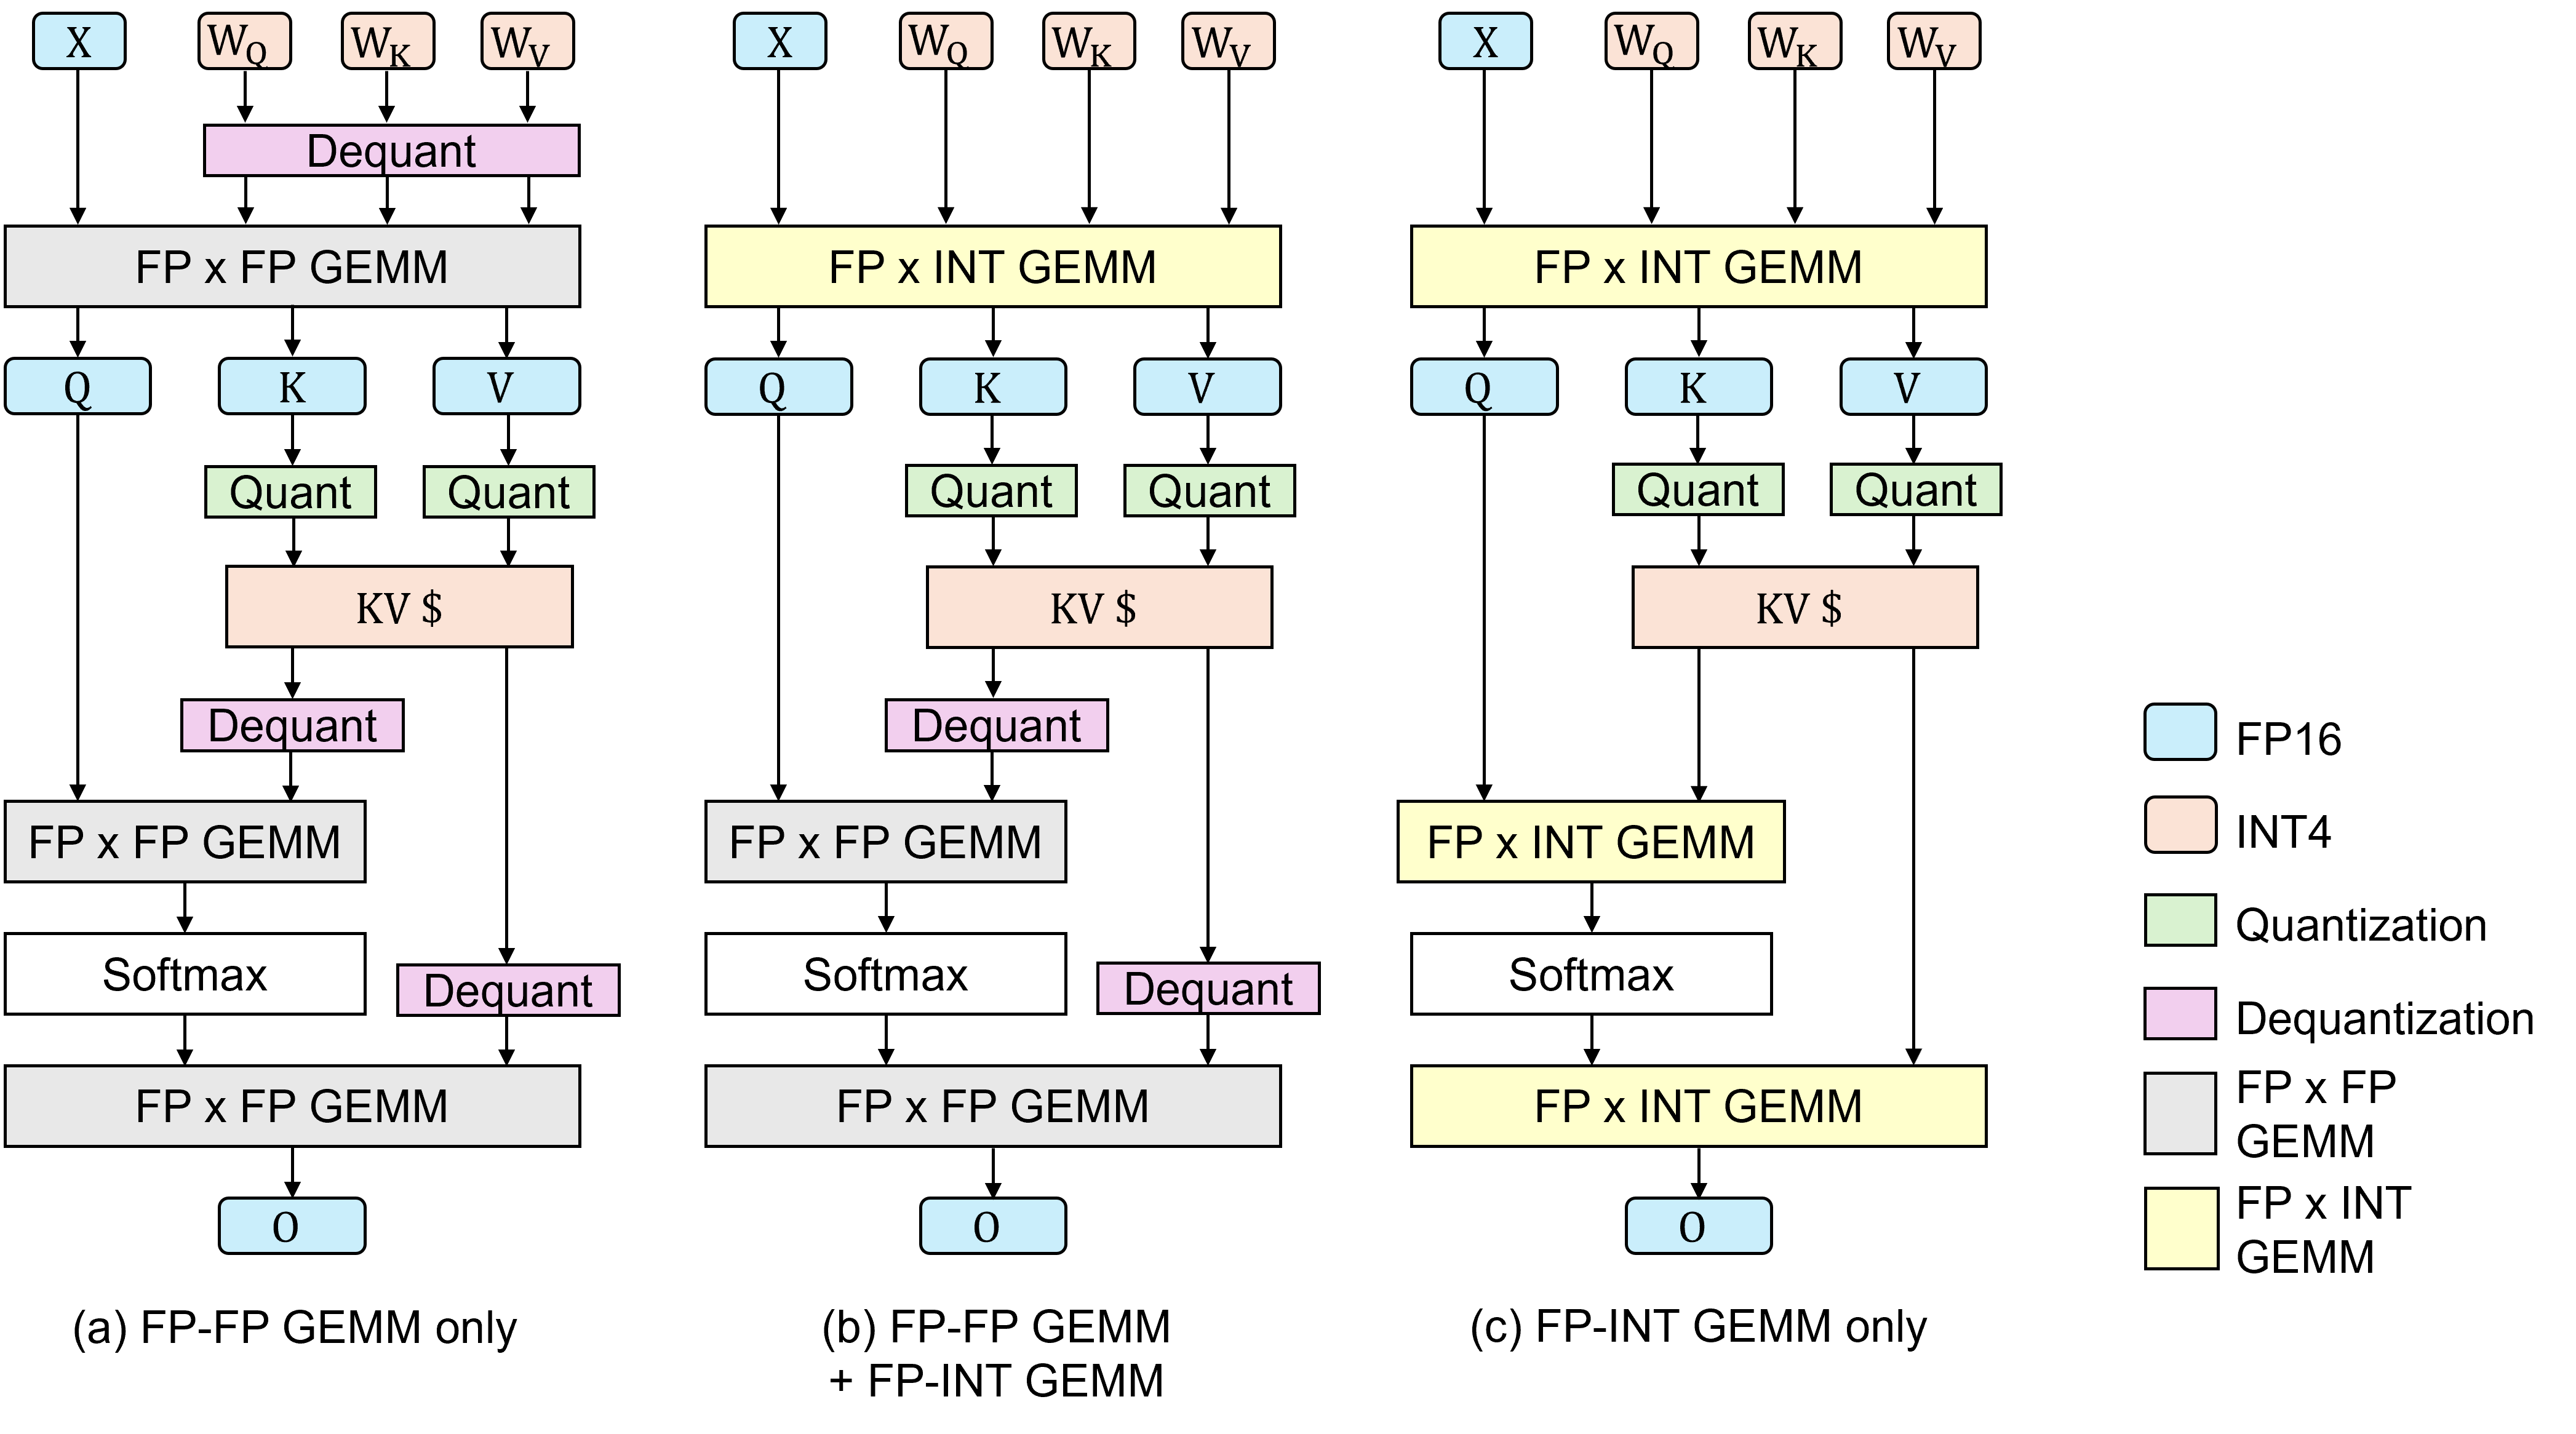
\includegraphics[width=0.98\linewidth]{figures/FIGS_figure1.png}
    \caption{Execution paths for WKV quantized inference: (a) conventional GPU dequantizes INT weight/KV operands before FP GEMM, (b) prior \fpint{} hardware accelerates linear layers but leaves quantized KV attention on the FP path, and (c) our design executes both linear and attention GEMMs using native \fpint{} paths.}
    \label{fig:fpint_inference}
\end{figure}

\subsection{Why Memory Saving Alone is Insufficient}

The most direct benefit of quantization is a reduction in memory footprint. However, as serving environments move toward high batch size or long sequence length, compute demand grows rapidly. The prefill stage processes a long prompt in one shot and is generally compute-bound. The generation stage runs token-by-token, so KV-cache traffic dominates and it is often memory-bound; yet structures such as GQA, MQA, and MLA reduce the number of KV heads or the KV representation and can push generation closer to a compute-bound regime, so computation cannot be considered unimportant (Figure~\ref{fig:bottleneck-analysis}). Reducing memory traffic alone is therefore no longer sufficient for modern LLMs; a compute path that processes quantized operands directly on a high-efficiency datapath, without dequantization, is required.

\begin{figure}[t]
    \centering
    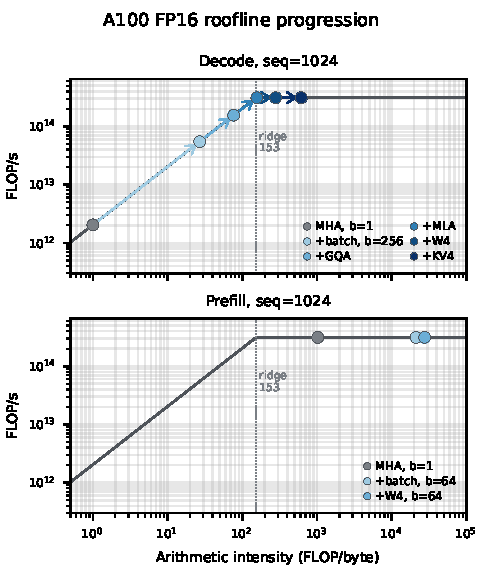
\includegraphics[width=0.92\linewidth]{figures/progression_roofline.pdf}
    \caption{Memory traffic reduction alone becomes insufficient as arithmetic intensity increases.}
    \label{fig:bottleneck-analysis}
\end{figure}

\subsection{Software mpGEMM Optimization and Its Limitation}

Software-based quantized GEMM kernels fuse dequantization with GEMM to reduce memory movement and raise Tensor Core utilization. This approach has the advantage of being deployable on existing GPUs immediately. However, this preserves the underlying structure, in which INT operands are converted to FP and then computed on an FP Tensor Core. From a latency perspective, dequantization can be overlapped, but from a TOPS and energy perspective, clear limits remain. On the energy side, both the dequantization itself and the high MAC cost of the FP$\times$FP TCU persist. In large-scale LLM serving systems where power delivery is becoming the data-center bottleneck, energy efficiency is no longer a factor that can be ignored. On the TOPS side, because an area-heavy FP$\times$FP TCU is still used, the additional throughput that an \fpint{} unit could otherwise provide is left on the table. Even when latency hiding lets the TCU run well, throughput could grow further if the TCU had more MACs; the FP$\times$FP TCU loses this opportunity because its TOPS/mm$^2$ is lower than that of an \fpint{} unit. Prior work on \fpint{} GEMM units reports a roughly $2$--$9\times$ improvement in both TOPS/mm$^2$ and TOPS/W over an FP$\times$FP unit, depending on the format~\cite{figna}. For high-throughput LLM serving, software optimization alone therefore has a hard ceiling on both performance and energy efficiency, and native \fpint{} hardware support is required.

\subsection{Hardware mpGEMM Accelerator and System-Level Gap}
\label{sec:sys_gap}

Prior mixed-precision hardware studies use custom arrays or lookup-table-based units to perform FP-to-INT multiplications efficiently. They show high TOPS/mm$^2$ and TOPS/W at the array level, but three gaps remain before these gains translate into end-to-end LLM-inference performance.

\textbf{Gap 1: \fpint{} native attention cannot be supported at the prefill or generation stage.}
KV quantization has traditionally been used to shrink the KV cache at the generation stage, and because conventional GPUs only carry FP$\times$FP units, KV-cache quantization is not used to accelerate GEMM in prefill --- it is actually treated like a post-processing overhead (Figure~\ref{fig:prefill_difference}). However, since the compute volume in the prefill attention grows as $O(N^2)$ with sequence length, attention comes to occupy a substantial fraction of TTFT in long-sequence regimes (Figure~\ref{fig:long_seq_atten_overhead}). Exploiting KV quantization to accelerate GEMM during prefill is therefore a very promising avenue for reducing TTFT.

The problem is that, due to limitations of their GEMM units, prior designs ignore the GEMMs inside attention and accelerate only the \fpint{} GEMMs of the linear layers. As a result, KV quantization is not used at all to reduce TTFT in prefill, and the end-to-end gains in the long-sequence regime are severely limited.

\begin{figure}[t]
    \centering
    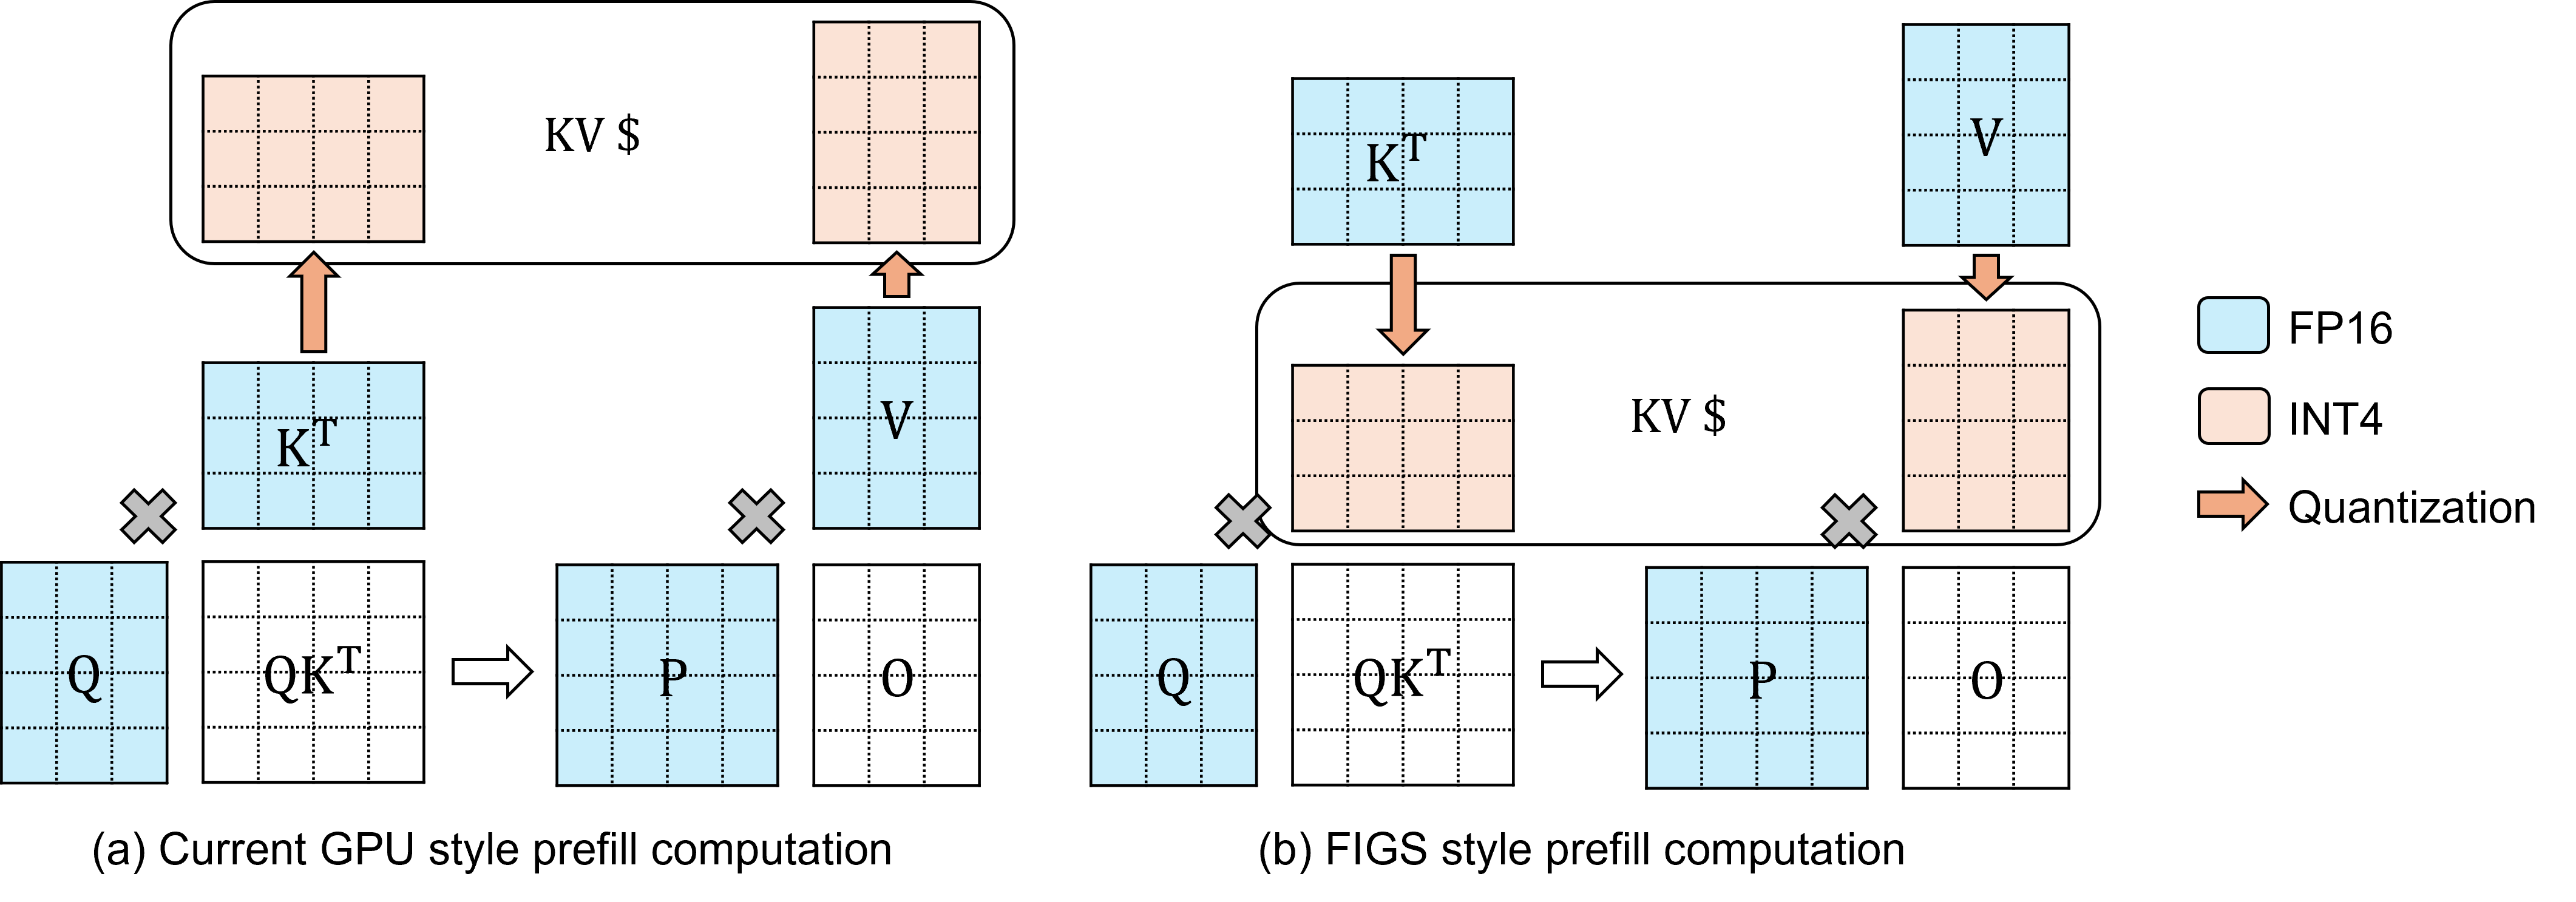
\includegraphics[width=0.92\linewidth]{figures/FIGS_figure_prefill.png}
    \caption{Current GPUs execute prefill with KV in FP16, while our design quantizes KV to INT4 and computes attention directly on quantized KV.}
    \label{fig:prefill_difference}
\end{figure}

\begin{figure}[t]
    \centering
    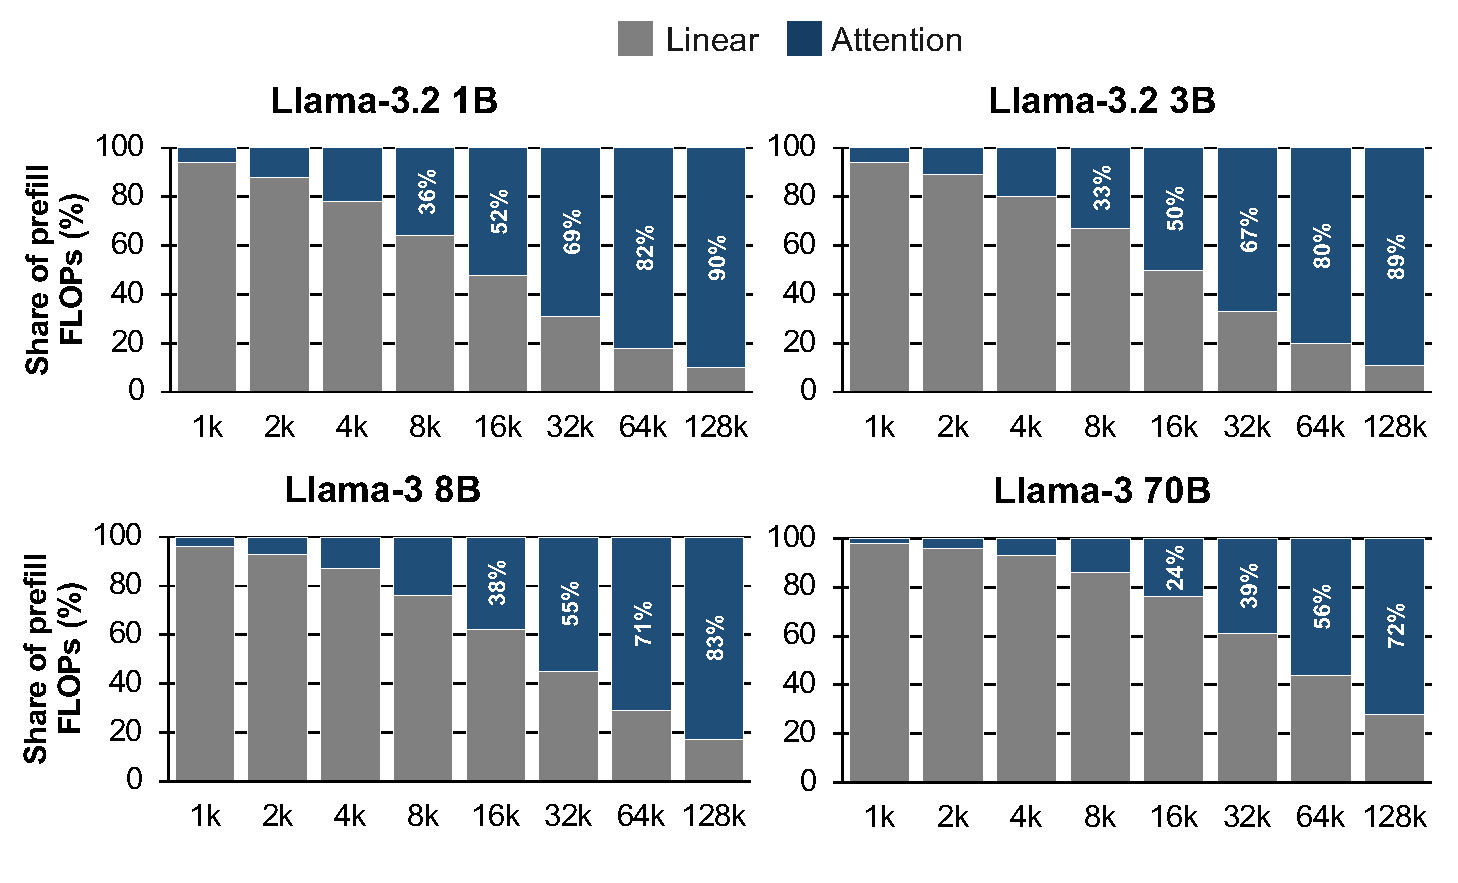
\includegraphics[width=0.92\linewidth]{figures/long_seq_attn_breakdown.pdf}
    \caption{Accelerating attention becomes critical in the long-sequence regime.}
    \label{fig:long_seq_atten_overhead}
\end{figure}

The first reason prior work does not support \fpint{} attention is that the quantization direction of the KV cache is not friendly to the compute units of prior mixed-precision accelerators. When we collate the K/V quantization directions used by common quantization frameworks, the directions are not uniformly fixed to token-wise or head-wise for both K and V, and they often differ across frameworks (Table~\ref{tab:kv_quant_granularity})~\cite{liu2024kivi,hooper2024kvquant,he2024zipcache,yue2024wkvquant,duanmu2024skvq,ashkboos2024quarot,liu2024spinquant}.

\begin{table}[t]
\centering
\caption{Quantization granularity of KV-cache quantization schemes.}
\label{tab:kv_quant_granularity}
\begin{tabular}{p{0.4\linewidth}p{0.25\linewidth}p{0.20\linewidth}}
\toprule
Scheme & K Direction & V Direction \\
\midrule
KIVI / KVQuant / ZipCache & channel & token \\
WKVQuant / SKVQ & token & token \\
QuaRot / SpinQuant & token / channel & token \\
\bottomrule
\end{tabular}
\end{table}

When K is channel-wise or V is token-wise, every element along the reduction dimension of the GEMM carries a different scale factor. Handling this on the GEMM units of existing mixed-precision accelerators prevents the use of an INT reduction tree, since each INT multiplication must be dequantized to FP and an additional FP reduction is then required, which destroys the original efficiency (Figure~\ref{fig:quant_row_dir_overhead}).

\begin{figure}[t]
    \centering

    \begin{subfigure}[t]{\linewidth}
        \centering
        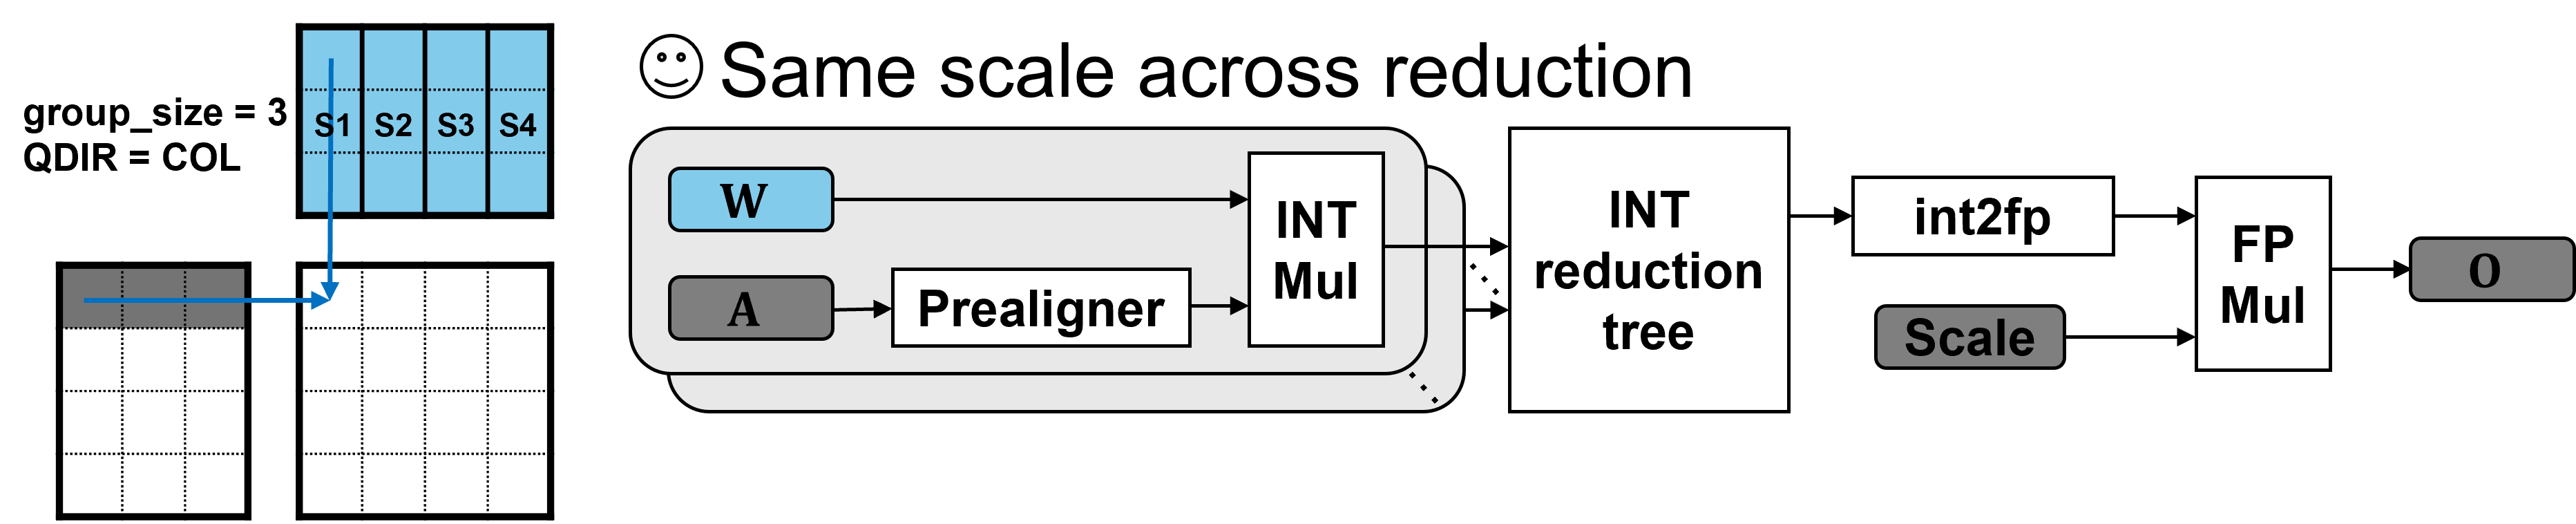
\includegraphics[width=0.92\linewidth]{figures/figs_fig5_4_a.png}
        \caption{Quant direction column (FIGNA style).}
        \label{fig:conv_acc}
    \end{subfigure}

    \vspace{0.5em}

    \begin{subfigure}[t]{\linewidth}
        \centering
        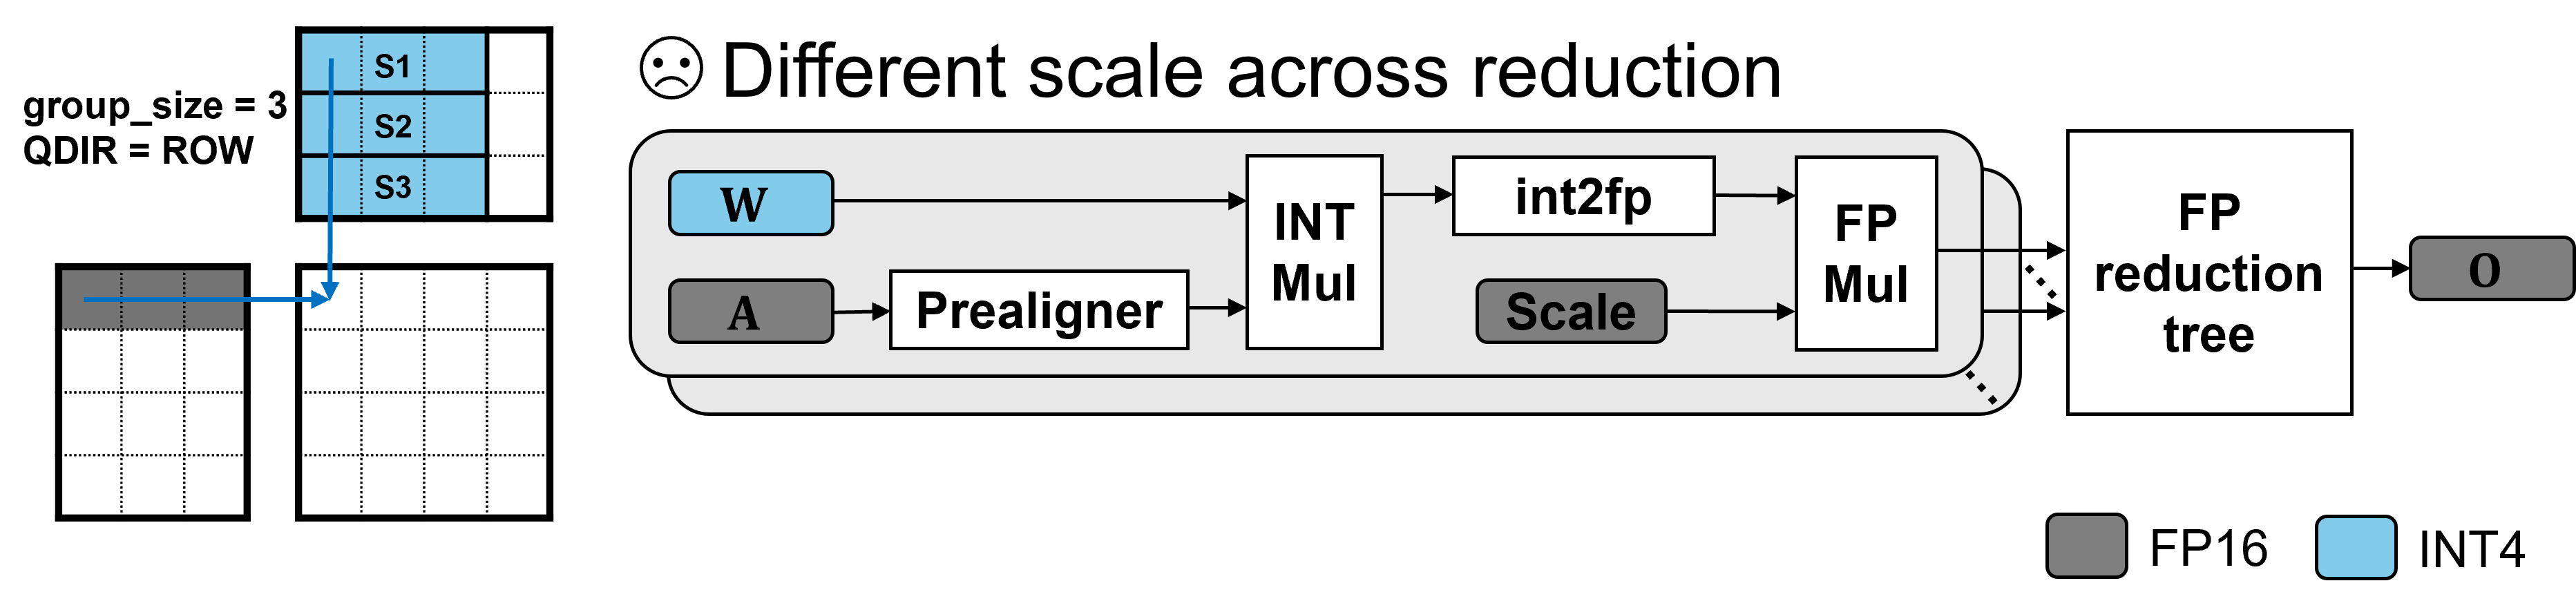
\includegraphics[width=0.92\linewidth]{figures/figs_fig5_4_b.png}
        \caption{Quant direction row (FIGNA style).}
        \label{fig:row_quant}
    \end{subfigure}

    \caption{Row-direction quantization introduces overhead when executed on a conventional accelerator structure.}
    \label{fig:quant_row_dir_overhead}
\end{figure}

\textbf{Gap 2: A larger MXU alone does not guarantee performance gains.}
Simply exploiting the high TOPS/mm$^2$ of an \fpint{} unit to pack a larger MXU into the same area does not, by itself, guarantee system-level performance gains. To convert TOPS/mm$^2$ into higher delivered TOPS, the MXU must keep its utilization high even as the MAC count grows; prior mixed-precision accelerators work concentrates on array-level performance and does not study utilization at the full-system level in depth.

Sustaining MXU utilization requires two things. First, the peak bandwidth of the memory subsystem must scale together with the enlarged MXU. Second, this scaled memory subsystem must be exercised in a low-latency, bursty fashion.

Scaling the bandwidth of the memory subsystem is harder than it appears. Conventional GPU-style memory hierarchies expose general-purpose access across the entire memory subsystem (shared memory, cache, and the register file) and therefore rely heavily on crossbars~\cite{jin2024uncovering, tine2021vortex}. As a result, replacing an FP$\times$FP MXU with an \fpint{} MXU while keeping the crossbar-based architecture and naively scaling the memory subsystem causes the crossbar cost to grow as $O(N^2)$, so the TOPS/mm$^2$ advantage almost vanishes at the system level, and in the worst case TOPS/mm$^2$ actually decreases (Figure~\ref{fig:xbar_overhead}).

A common way to scale memory-subsystem bandwidth is to increase the number of banks and use an interleaving address scheme. The catch is that designing a DMA that fully exploits this bandwidth is far from trivial. Every burst request must respect the constraint that the data it fetches in a single transaction do not cross a bank boundary. Misaligned accesses additionally require a barrel shifter, and as the data width of the DMA scales up the barrel shifter must scale with it; handling a misaligned access in a single cycle then incurs significant area, power, and timing overhead.

In short, increasing bandwidth is non-trivial due to the crossbar cost, and even when bandwidth is scaled, exploiting it requires the DMA to burst while satisfying two constraints simultaneously: every per-cycle request must stay within a bank boundary, and misaligned accesses must be avoided.

\begin{figure}[t]
    \centering
    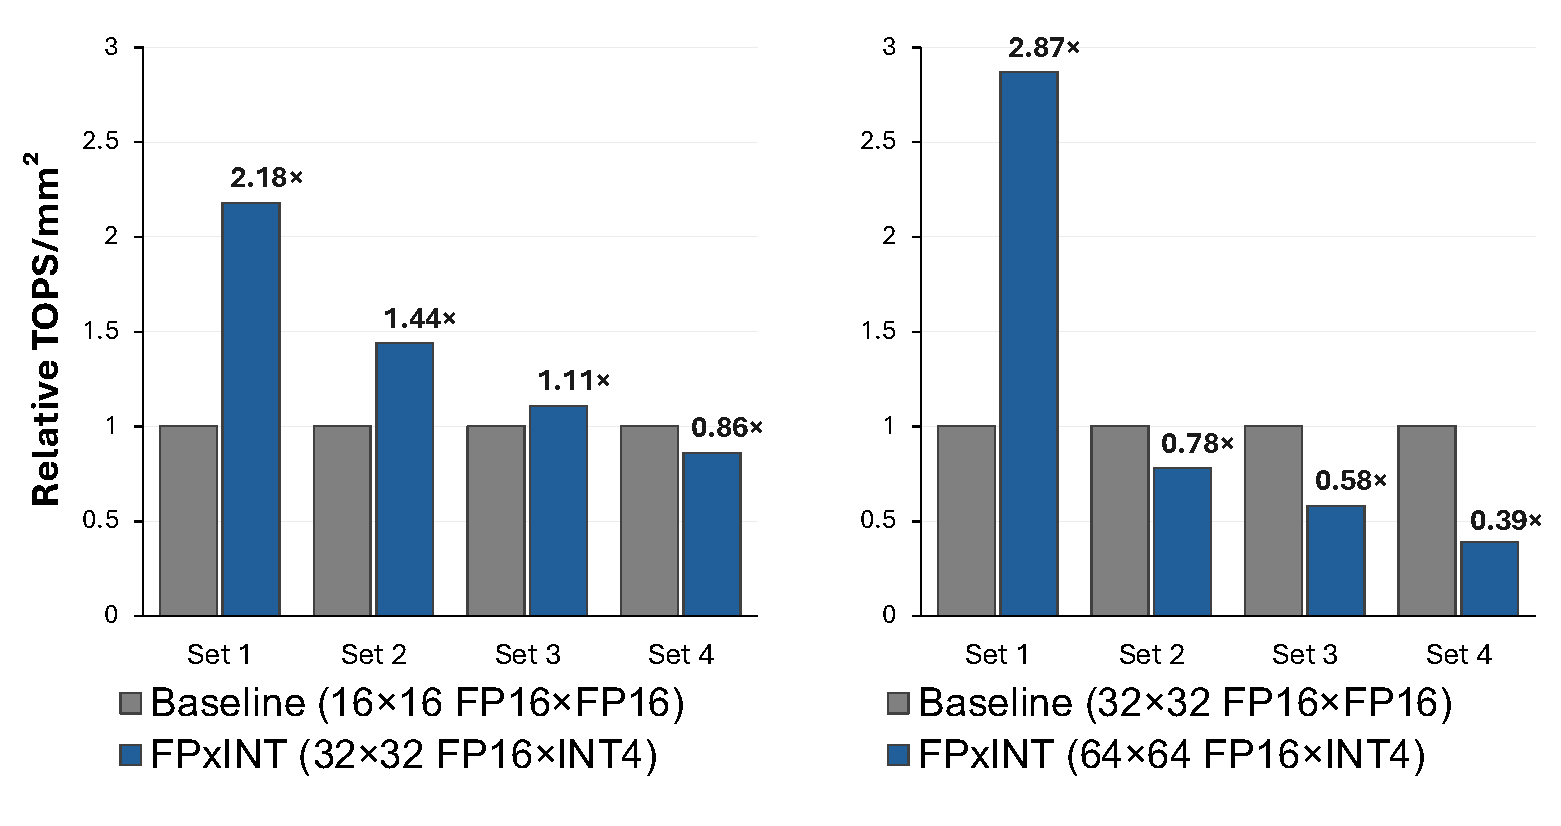
\includegraphics[width=0.98\linewidth]{figures/xbar_overhead_value.pdf}
    \caption{Relative TOPS/mm$^2$ of FPxFP vs.\ FPxINT GEMM arrays with progressively included memory-system area overheads. Bars are normalized to the FPxFP baseline for each set, with absolute area shown in-bar. GEMM area includes its own PnR; Set~4 includes memory-system PnR. CAP-intrinsic SRAM area is excluded, while SRAM peripheral overhead is charged only to FPxINT. L/D/A are LMEM banks/requests, DCACHE banks/requests/ports, and AXI input ports, set by $L=N^2/16$, $D=A=\max(1, N^2/128)$.}
    \label{fig:xbar_overhead}
\end{figure}

\section{FIGS Design Overview}

\begin{figure*}[t]
    \centering
    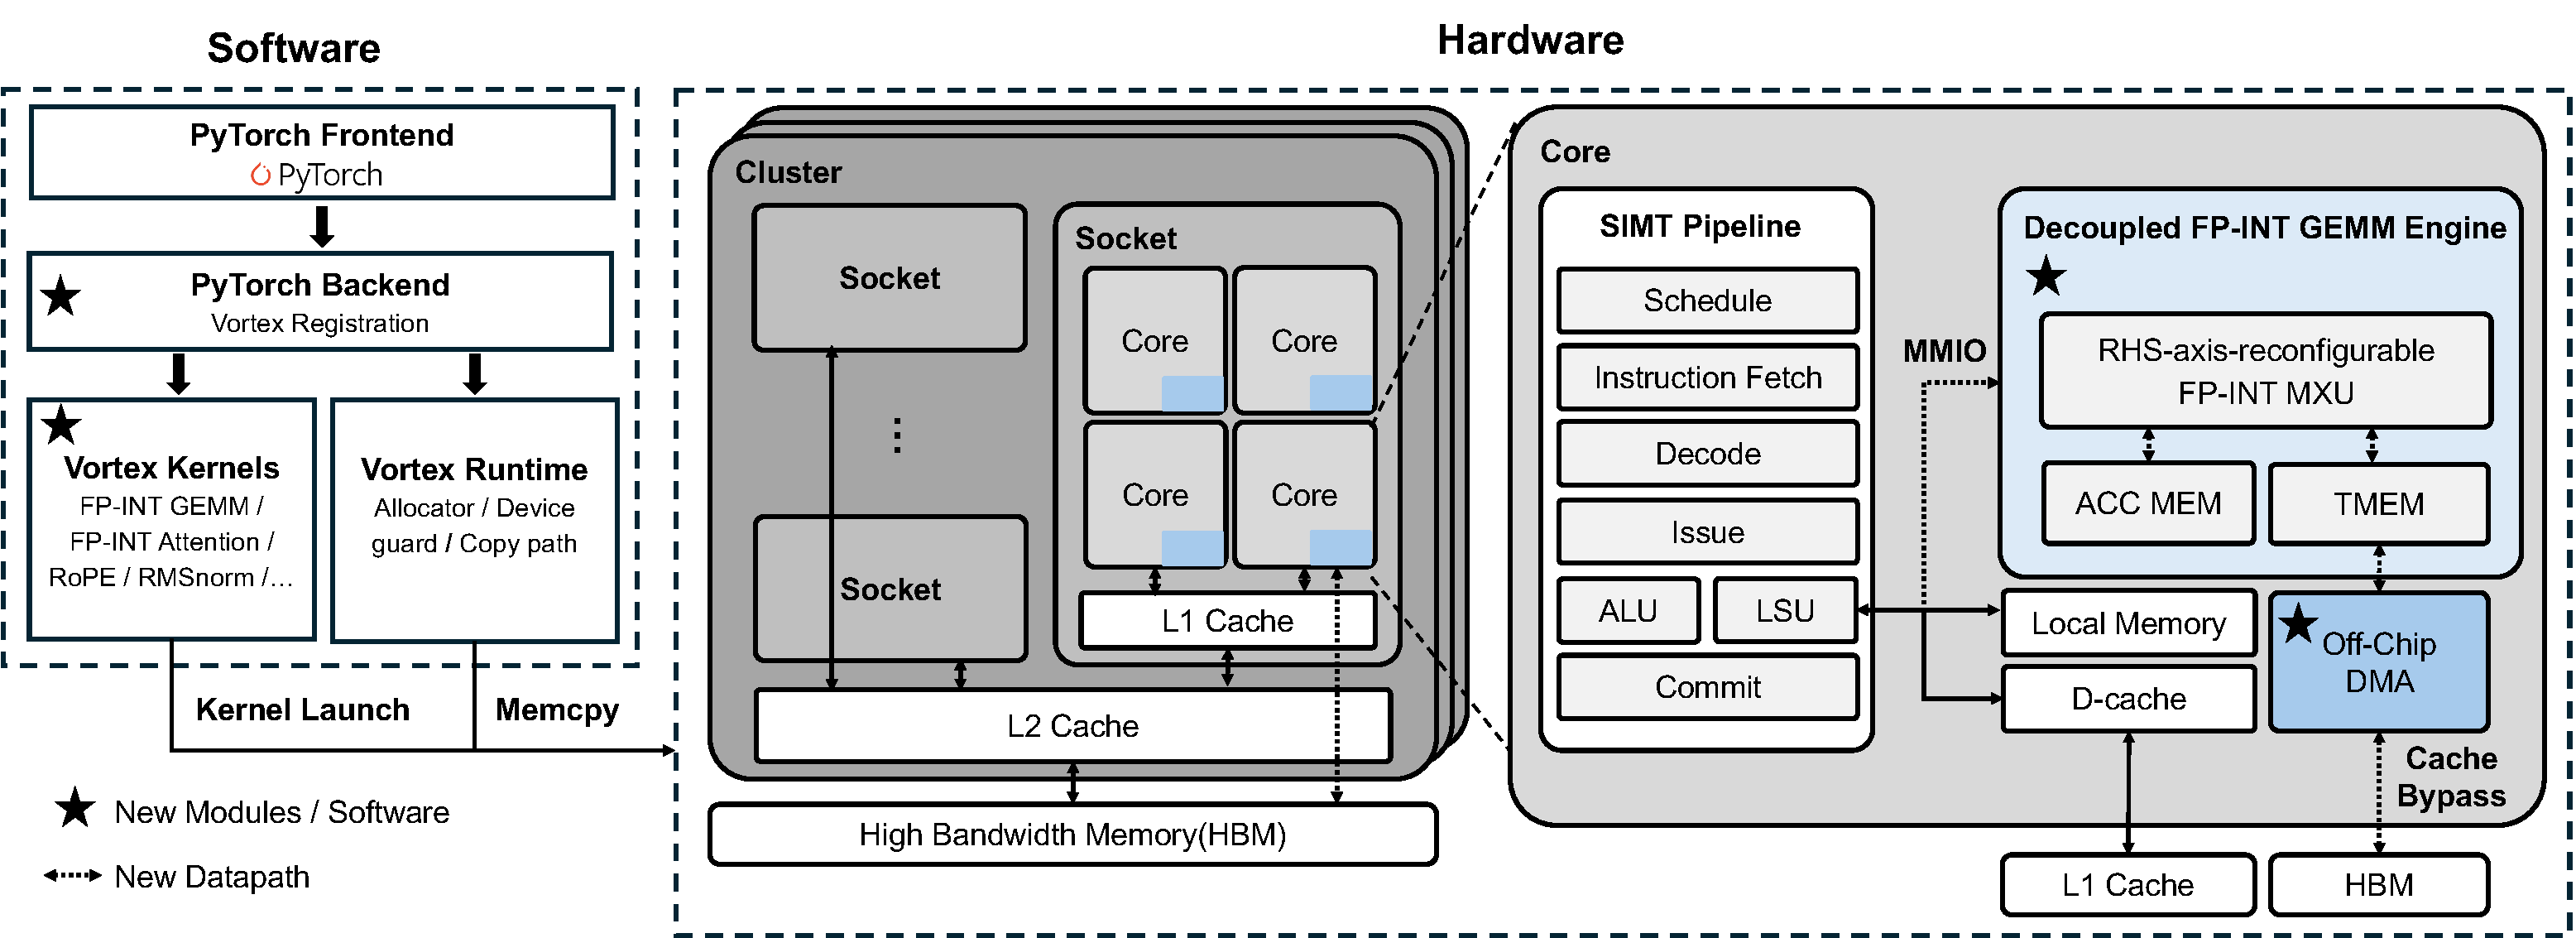
\includegraphics[width=0.95\linewidth]{figures/fig7.pdf}
    \caption{Overview of the proposed hardware/software system.}
    \label{fig:overview}
\end{figure*}

\ours{} is a system built on top of Vortex\cite{tine2021vortex}, an open-source GPGPU, that accelerates WKV-quantized models by integrating an \fpint{} GEMM engine together with a low-cost memory subsystem and a software stack designed to keep that engine at maximum utilization.
Figure~\ref{fig:overview} shows the high-level organization of \ours{}.
The original Vortex SIMT pipeline remains responsible for control flow, vector operations, kernel launch, and synchronization, while a decoupled \fpint{} GEMM engine executes the linear and attention GEMMs through MMIO-issued descriptors.
Tensor operands move between HBM pseudo-channels, tensor memory, and the GEMM engine through a cache-bypassed direct tensor path, and the runtime/software stack manages layout, alignment, and synchronization so that this restricted path can be used efficiently.
To make this system effective end-to-end, we make several design decisions.

\textbf{Retaining the Vortex SIMT pipeline.}
An LLM contains a variety of vector operations in addition to GEMM. Even though these vector operations carry a small fraction of the total work, falling back to a CPU for them would incur a large overhead. We therefore keep the SIMT pipeline to preserve programmability and generality.

% \paragraph{The \fpint{} GEMM engine must support every combination of the RHS quantization direction and the load direction.}
\textbf{Reconfigurable RHS quantization and load direction.}
The \fpint{} GEMMs that appear repeatedly in a \wkv{} quantized model vary along two axes: the quantization direction of the RHS matrix, and whether the RHS is transposed. In QK$^T$, the RHS must be consumed in transposed form, whereas in PV, the linear projections, and the FFN, the RHS is non-transposed. As Table~\ref{tab:kv_quant_granularity} shows, the KV quantization can be either token-wise or channel-wise. To fully accelerate a WKV-quantized model, the \fpint{} GEMM engine must therefore support all four execution patterns in a reconfigurable manner.

% \paragraph{We decouple the GEMM engine from SIMT and use dedicated tensor memory and accumulator memory.}
\textbf{Decoupled GEMM engine with dedicated tensor and accumulator memory.}
The most commonly cited problem of a TCU is register pressure, and this problem grows worse as the TCU becomes larger. Because the \fpint{} GEMM engine leverages high TOPS/mm$^2$ to instantiate a large MXU, coupling it to the SIMT core would prevent us from sustaining high utilization due to register pressure. \ours{} therefore decouples the GEMM engine from the SIMT core. Using the GPU shared memory as the communication path between the engine and the cores is not attractive either: the shared memory is interconnected through a crossbar, so its bandwidth is hard to scale, and conflicts with SIMT load/store instructions can lower the engine's utilization. We therefore carve out a portion of the shared-memory capacity as a separate tensor memory that forms an independent memory space. In addition, in a quantized model the partial-sum bitwidth is larger than that of the inputs and weights because of dequantization. Placing a dedicated accumulator memory inside the GEMM engine avoids spending input/weight bandwidth on partial-sum traffic and lets us guarantee conflict-freedom at the dataflow level. As a result, we can run the GEMM at full throughput on single-port SRAMs using a word-wise ping-pong scheme inside the engine, without ever asserting a back-pressure signal.

% \paragraph{The GEMM command stream is generated by a hardware micro-op FSM, not by a software queue.}
\textbf{Hardware-generated GEMM command stream.}
A large \fpint{} MXU demands not only operand bandwidth but also command bandwidth, which a software-built command queue cannot sustain. Our initial design had the kernel build tile-level commands through bit manipulation and enqueue them into a command queue via store instructions, with the hardware decoding them downstream. On the Vortex-based GPU used in this paper, however, the scalar command stream produced by a single warp was not fast enough, and command packing and queue stores became the bottleneck of the GEMM launch path. \ours{} instead has the kernel program the matrix shape, stride, tensor/accumulator base addresses, qdir, load direction, and scale/zero-point metadata into MMIO registers, and submit the request through a doorbell. Once a request slot is successfully allocated, a micro-op generation FSM inside the GEMM engine expands the descriptor into DMA, RHS load, MXU step, accumulator update, and completion signaling. In other words, the SIMT pipeline only handles compact descriptor setup and synchronization, while the repetitive GEMM micro-op stream is produced by a hardware sequencer.

% \paragraph{Rather than scaling the memory subsystem with a complex crossbar, we scale it at low cost with a simple interconnect fabric and handle the resulting constraints in the software stack.}
\textbf{Crossbar-less interconnect with software-handled constraints.}
Naively scaling memory-subsystem components that contain a crossbar actually degrades TOPS/mm$^2$. To avoid this, \ours{} connects HBM pseudo-channels, tensor-memory banks, and GEMM-engine lanes without any crossbar. The tensor traffic on these connections travels along a separate DMA path that does not pass through the cache hierarchy. This choice avoids the crossbar cost that would arise when scaling the cache/local-memory interconnect to the operand bandwidth of the \fpint{} engine. The correctness issue introduced by this non-coherent bypass path is not resolved by a hardware protocol that supports arbitrary sharing; instead, it is handled by phase-based buffer ownership and explicit synchronization in the GEMM kernel. When the source and destination components have the same count, we use a 1:1 connection; otherwise we use a simply interleaved connection. The side effect of removing the crossbar is that constraints on data movement appear --- for example, data at HBM address X may not always be movable to TMEM address Y. For GEMM, the regular dataflow makes these constraints simple enough that the software stack (compiler, runtime, and kernel design) can satisfy them without much effort. As a result, we scale the memory bandwidth by $8\times$ with only about a 3\% increase in total area.

\section{Native \fpint{} Attention Support}

As discussed in Section~\ref{sec:sys_gap}, executing the attention of a \wkv{} quantized model as a native \fpint{} GEMM requires more than an MXU that simply multiplies an FP operand with an INT operand. The core difficulty is that the tensor axis to which the quantization metadata of the INT RHS operand is bound conflicts directly with the reduction, accumulation, and transpose directions of the GEMM dataflow. In weight quantization, scales and zero points are typically fixed along the output channel or group, so the INT dot product can be carried out first and dequantization can then be applied at the granularity of an output tile. In KV-cache quantization, by contrast, the scale may be defined token-wise, channel-wise, or group-wise, and even the same metadata axis is mapped to different GEMM directions for QK$^T$ and PV. As a result, a conventional \fpint{} MXU can apply the scale after accumulation in some cases, but in others must apply it to every product term before accumulation. The latter case forces a per-term FP multiplication and an FP reduction across terms, or falls back to an FP path for attention, eliminating the compute-side benefit of \wkv{} quantization.

To address this, we propose an RHS-axis-reconfigurable \fpint{} MXU in which the RHS quantization direction and the RHS load direction can be reconfigured independently. The proposed MXU selects one of two execution modes, QCOL and QROW, according to the qdir configuration. The difference between the two modes can be summarized as where the same \fpint{} GEMM applies the scale and the zero point. In the following, $A$ is the FP input operand, $B^{int}$ is the INT RHS operand, $G_K$ and $G_N$ are the quantization group sizes along the reduction and output dimensions, $g(k)=\lfloor k/G_K \rfloor$, and $h(n)=\lfloor n/G_N \rfloor$.

In QCOL, the scale and the zero point are bound to the reduction group and the output column. Within a group, $S^{\mathrm{COL}}_{g,n}$ and $Z^{\mathrm{COL}}_{g,n}$ are invariant in the reduction index $k$, so output scaling can be deferred to the end of the dot product:
\begin{align}
    C^{\mathrm{COL}}_{m,n}
    &=
    \sum_g S^{\mathrm{COL}}_{g,n}
    \left(
        \sum_{k \in \mathcal{K}_g} A_{m,k} B^{int}_{k,n}
        -
        Z^{\mathrm{COL}}_{g,n} \sum_{k \in \mathcal{K}_g} A_{m,k}
    \right) .
    \label{eq:qcol-fpint}
\end{align}
The QCOL datapath therefore lets the MXU compute $\sum A B^{int}$ while the activation reduce tree computes $\sum A$; a zero-point multiplier then produces $-Z^{\mathrm{COL}}_{g,n}\sum A$, which is added to the MXU partial sum. In the post-processing stage, the output scaler finally multiplies by $S^{\mathrm{COL}}_{g,n}$. This dataflow is possible because the scale remains stationary along the output lane.

In QROW, by contrast, the scale and the zero point are bound to the reduction index and the output group. Since $S^{\mathrm{ROW}}_{k,h(n)}$ and $Z^{\mathrm{ROW}}_{k,h(n)}$ now change with $k$, multiplying by a single output scale after accumulation is no longer valid:
\begin{align}
    C^{\mathrm{ROW}}_{m,n}
    &=
    \sum_k A_{m,k}
    \left(
        S^{\mathrm{ROW}}_{k,h(n)} \cdot
        (B^{int}_{k,n} - Z^{\mathrm{ROW}}_{k,h(n)})
    \right) \\
    &=
    \sum_k \bar{A}^{(h)}_{m,k} B^{int}_{k,n}
    -
    \sum_k \bar{A}^{(h)}_{m,k} Z^{\mathrm{ROW}}_{k,h(n)},
    \label{eq:qrow-fpint}
\end{align}
where $\bar{A}^{(h)}_{m,k}=A_{m,k}S^{\mathrm{ROW}}_{k,h(n)}$.
In QROW mode, therefore, the scale is not left as RHS dequantization metadata; instead, it is folded into the FP input stream before it enters the MXU. After scale folding, the main product becomes a standard \fpint{} dot product of the form $\sum \bar{A} B^{int}$, and the output-side scaler is bypassed.

The zero-point correction path in hardware follows the same equations in a qdir-dependent order. Let the prealigner convert the FP input into the integer representation $\hat{A}$ consumed by the MXU. For notational simplicity, we absorb the fixed-point exponent and bit-shift correction into $\hat{A}$. In QCOL, the zero point varies only across columns within a group, so the activation sum is formed first and then multiplied by the per-column zero point:
\begin{align}
    P^{\mathrm{COL}}_{m,n} &= \sum_{k \in \mathcal{T}} \hat{A}_{m,k} B^{int}_{k,n}, \\
    R^{\mathrm{COL}}_{m} &= \sum_{k \in \mathcal{T}} \hat{A}_{m,k}, \\
    D^{\mathrm{COL}}_{m,n} &= (-Z^{\mathrm{COL}}_{g,n}) R^{\mathrm{COL}}_{m}, \\
    I^{\mathrm{COL}}_{m,n} &= P^{\mathrm{COL}}_{m,n} + D^{\mathrm{COL}}_{m,n} .
    \label{eq:qcol-correction}
\end{align}
In Figure~\ref{fig:fpint-gemm-unit}, this path corresponds to \texttt{prealigner} $\rightarrow$ \texttt{act\_reduce} $\rightarrow$ \texttt{zp\_mul} $\rightarrow$ \texttt{merger}.

In QROW, the zero point differs per reduction lane, so summing the activations first would lose track of which zero point should be multiplied. We therefore form the per-lane zero-point product first, using the prealigned scale-folded input $\hat{\bar{A}}$ obtained from $\bar{A}$, and reduce those products afterwards:
\begin{align}
    P^{\mathrm{ROW}}_{m,n} &= \sum_{k \in \mathcal{T}} \hat{\bar{A}}^{(h)}_{m,k} B^{int}_{k,n}, \\
    D^{\mathrm{ROW}}_{m,h} &= \sum_{k \in \mathcal{T}} (-Z^{\mathrm{ROW}}_{k,h}) \hat{\bar{A}}^{(h)}_{m,k}, \\
    I^{\mathrm{ROW}}_{m,n} &= P^{\mathrm{ROW}}_{m,n} + D^{\mathrm{ROW}}_{m,h} .
    \label{eq:qrow-correction}
\end{align}
This path corresponds to \texttt{input scaler} $\rightarrow$ \texttt{prealigner} $\rightarrow$ \texttt{zp\_mul} $\rightarrow$ \texttt{act\_reduce\_tree} $\rightarrow$ \texttt{merger}. The same reduce tree and zero-point multiplier are used in both modes, but the routing changes from reduce-then-multiply in QCOL to multiply-then-reduce in QROW. This change preserves the per-$k$ zero-point correction required by QROW while reusing the same INT-RHS MXU datapath.

Attention changes not only the quantization direction but also the logical orientation of the RHS. PV and linear GEMMs consume the RHS tile in the standard orientation, whereas QK$^T$ must feed the K tile to the MXU in transposed form. To support this, we duplicate the RHS load network so that the same MXU array supports both row-wise and column-wise loading. The transpose is thus absorbed into a load-time configuration rather than handled by a separate memory-transform kernel. As shown in Figure~\ref{fig:fpint-gemm-unit}, the proposed unit provides a qdir-controlled scale/correction datapath together with a load-direction-controlled RHS injection path. The upper-level architecture only needs to set qdir, load direction, and the post-processing bypass flag for each linear, QK$^T$, or PV kernel, while the physical \fpint{} MXU array is shared across all paths.

The \texttt{DLY} block in Figure~\ref{fig:fpint-gemm-unit} is an FF-based delay element that matches the pipeline latency between the main product path and the correction path, both of which vary with qdir and load direction. With \texttt{DLY}, the \texttt{merger} and the accumulator stage receive cycle-aligned partial results. The \texttt{ACC MEM BANK} is dedicated storage for partial-sum accumulation. Instead of a true dual-port SRAM, it uses two single-port SRAM banks scheduled in a 1-cycle skewed ping-pong fashion: while one bank is read in a given cycle, the other is written, constraining the dataflow so that the two single-port banks behave as a logically dual-port accumulator bank.

\begin{figure}[t]
    \centering
    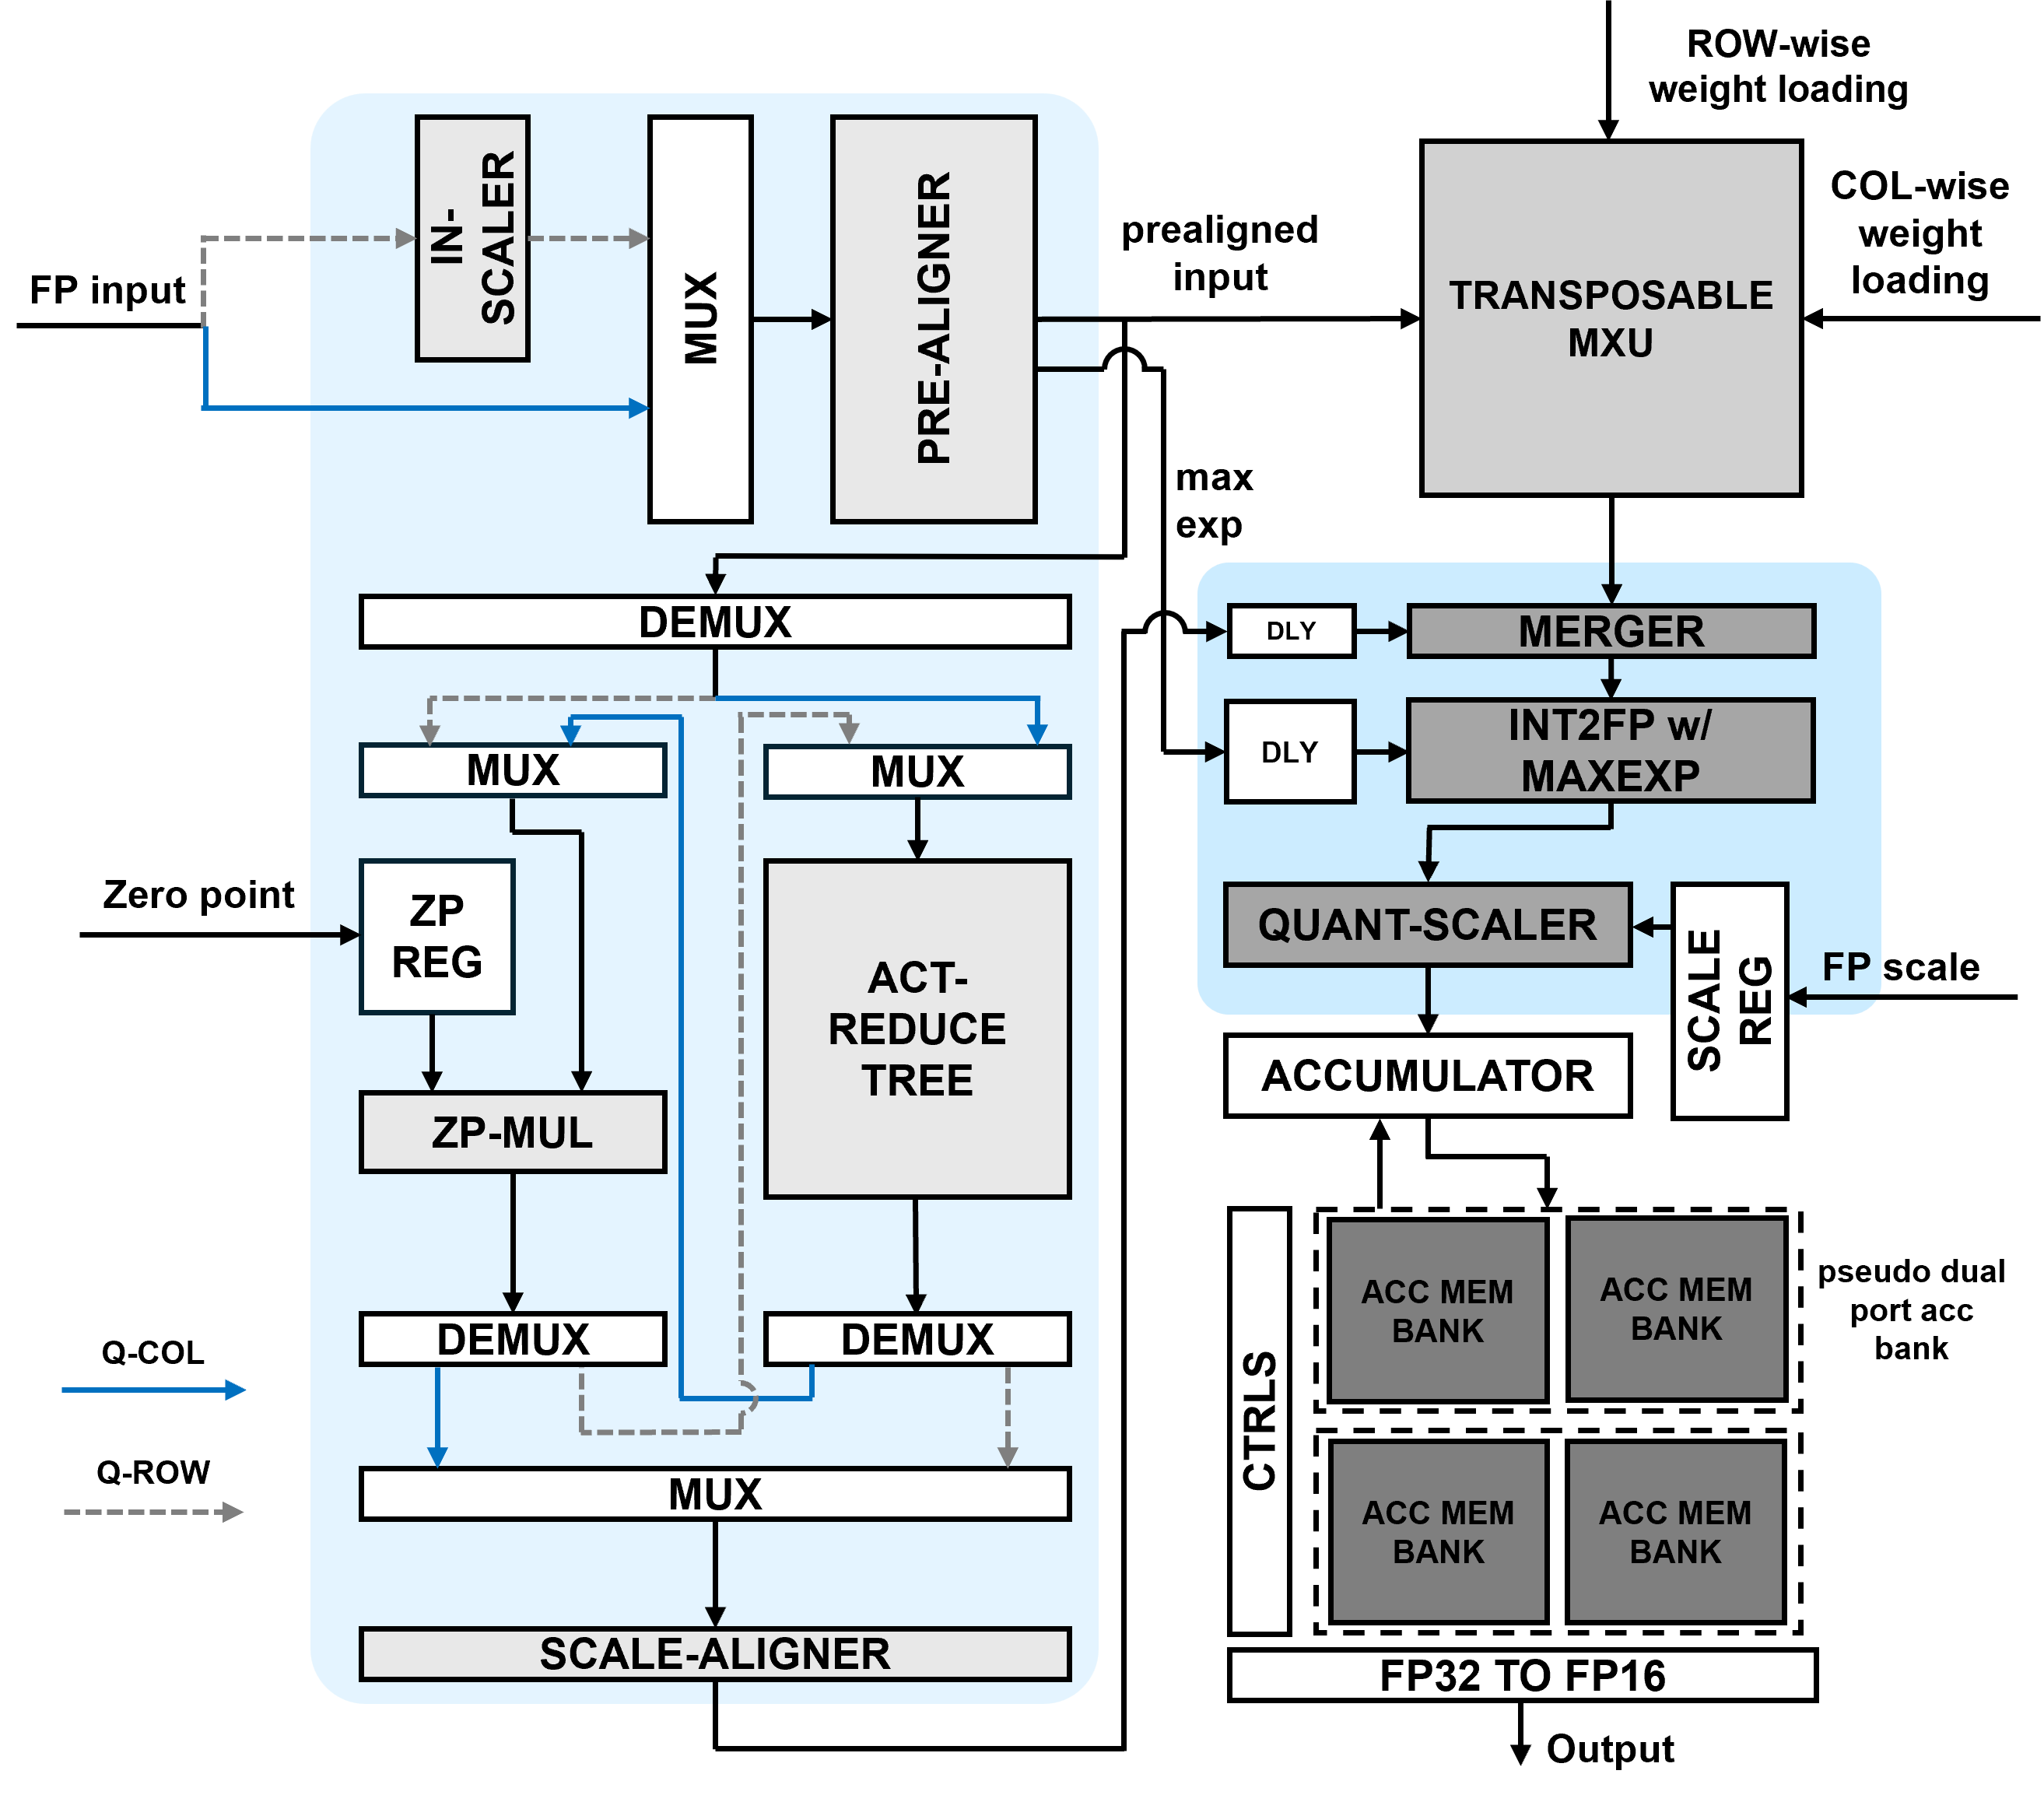
\includegraphics[width=0.92\linewidth]{figures/figs_fig8.png}
    \caption{RHS-axis-reconfigurable \fpint{} GEMM unit with scale-folding datapath and dual RHS load paths.}
    \label{fig:fpint-gemm-unit}
\end{figure}

The key effect of this design is the elimination of FP fallback in quantized attention. When only the linear layers are accelerated with \fpint{}, attention re-emerges as the bottleneck in long-context workloads. The proposed MXU, in contrast, executes both QK$^T$ and PV as native \fpint{} GEMMs, accelerating the main GEMM paths of a \wkv{} quantized model end-to-end from the linear layers all the way through the attention layers.

\section[Memory System for Sustained FP-INT Utilization]{Memory System for Sustained \fpint{} Utilization}
\label{sec:memory-system}

An \fpint{} MXU can provide more MACs than an FP$\times$FP Tensor Core at smaller area and lower energy. The accompanying increase in MAC density, however, directly translates into a higher operand bandwidth demand. If all operands are supplied through the register file, shared memory, and cache as in a conventional GPU-style datapath, the crossbar, arbitration, and routing costs grow rapidly as the port and bank counts increase. The memory system of \ours{} therefore does not simply attach the \fpint{} array next to the core; instead, it is designed to separate the regular tensor traffic required by the array from the general-purpose memory path.

\textbf{Decoupled GEMM Execution:}
The proposed \fpint{} MXU is not driven by tensor instructions that are tightly coupled to the SIMT register file. The SIMT kernel issues a request in a warp-specialized fashion by writing the information required for a GEMM operation into a designated MMIO space and then writing to a doorbell register. Once the GEMM command is successfully issued, a micro-op generation FSM inside the GEMM engine expands the descriptor into a tile-level sequence, and the DMA and the local DMA receive those commands and move data from HBM to TMEM and from TMEM into the GEMM engine. This organization avoids tying a large MXU to register-file bandwidth and warp-level operand scheduling, and thanks to a simple interconnect fabric it sustains sufficient bandwidth at low cost. The SIMT pipeline handles launch, synchronization, and non-GEMM vector operations, while the GEMM engine independently makes progress on long-running tensor operations.

\textbf{Partitioned On-Chip Tensor Storage:}
Local memory must retain flexible access for conventional load/store, inter-thread communication, and scalar/vector kernels. The GEMM operand stream, on the other hand, has a fixed tile shape and access order, so banked bandwidth matters more than full flexibility. \ours{} therefore partitions the on-chip SRAM into a general-purpose local memory and an MXU-dedicated tensor memory and accumulator memory. The tensor memory and the accumulator memory increase their bank count and data width under the assumption of a restricted access pattern, while the local memory preserves the existing SIMT programming model. In addition, since partial sums have a larger bitwidth than the operands and exhibit a different access pattern, they are stored in a separate accumulator memory inside the GEMM engine. This separation prevents input/weight bandwidth from interfering with partial-sum read-modify-write traffic, and it allows us to remove the ready signal of the valid-ready protocol on the deeply pipelined GEMM datapath, minimizing control overhead.

\textbf{Direct-Connected Tensor Data Path:}
Connecting HBM pseudo-channels to tensor memory banks via a fully connected crossbar allows bandwidth to be used flexibly, but the area and routing overheads grow super-linearly rather than proportionally to bandwidth. Figure~\ref{fig:memory-system} shows the memory subsystem for the case where the data width of HBM and the TMEM banks is 64\,B, the number of pseudo-channels and the number of TMEM banks are both 8, and the input precision is FP16. Here, $R_{\mathrm{MXU}}$ denotes the row dimension of the MXU, i.e., the number of reduction lanes consumed by the GEMM engine for a single input slice, which is 32 in Figure~\ref{fig:memory-system}. The memory subsystem of \ours{} connects HBM--TMEM and TMEM--MXU with a 1:1 or interleaved mapping, eliminating the all-to-all fabric. The interleaved scheme, for example, connects 4 source ports to 8 destination ports such that destination port $i$ is connected to source port $i \bmod 4$. This path lowers hardware cost at the price of a bank-mapping constraint between source and destination addresses. Specifically, when HBM pseudo-channels and TMEM banks both have a data width of $DW$ bytes and the numbers of pseudo-channels and TMEM banks are $\mathrm{NUM}_{pc}$ and $\mathrm{NUM}_{tmem}$, the addresses must satisfy
\begin{multline}
    \mathrm{Addr}_{\mathrm{HBM}}
    \equiv
    \mathrm{Addr}_{\mathrm{TMEM}} \\
    \pmod{DW \cdot \min\left(\mathrm{NUM}_{pc}, \mathrm{NUM}_{tmem}\right)} .
    \label{eq:hbm_tmem_addr_constr}
\end{multline}
Between TMEM and the GEMM engine, a base-address constraint arises at the granularity of the tensor slice that the GEMM engine consumes in one step. For instance, the GEMM engine of \ours{} reads the input slice $I[m, R_{\mathrm{MXU}} k : R_{\mathrm{MXU}}(k+1)-1]$ and feeds it into the internal MXU. The first element of this slice, $I[m, R_{\mathrm{MXU}} k]$, must always be aligned to the least-significant lane of the GEMM engine input port. To guarantee this, we restrict the TMEM addresses at which this element can be stored, which in turn simplifies the interconnect between TMEM and the GEMM engine. The base address of every slice consumed by the GEMM engine must therefore satisfy the following alignment constraint:
\begin{multline}
    \operatorname{Addr}_{\mathrm{TMEM}}
    \left(I\left[m, R_{\mathrm{MXU}} k\right]\right)
    \equiv 0 \\
    \pmod{
        \operatorname{lcm}
        \left(
            \operatorname{sizeof}(I) \cdot R_{\mathrm{MXU}},
            DW
        \right)
    } .
    \label{eq:tmem_gemm_addr_constr}
\end{multline}
While inconvenient for arbitrary memory copies, this constraint is easily met for the regular tensor traffic of GEMM tile movement through simple extensions to software layout transformation and memory allocation.

\textbf{Cache-Bypassed Tensor DMA:}
% \begin{figure}[t]
%     \centering
%     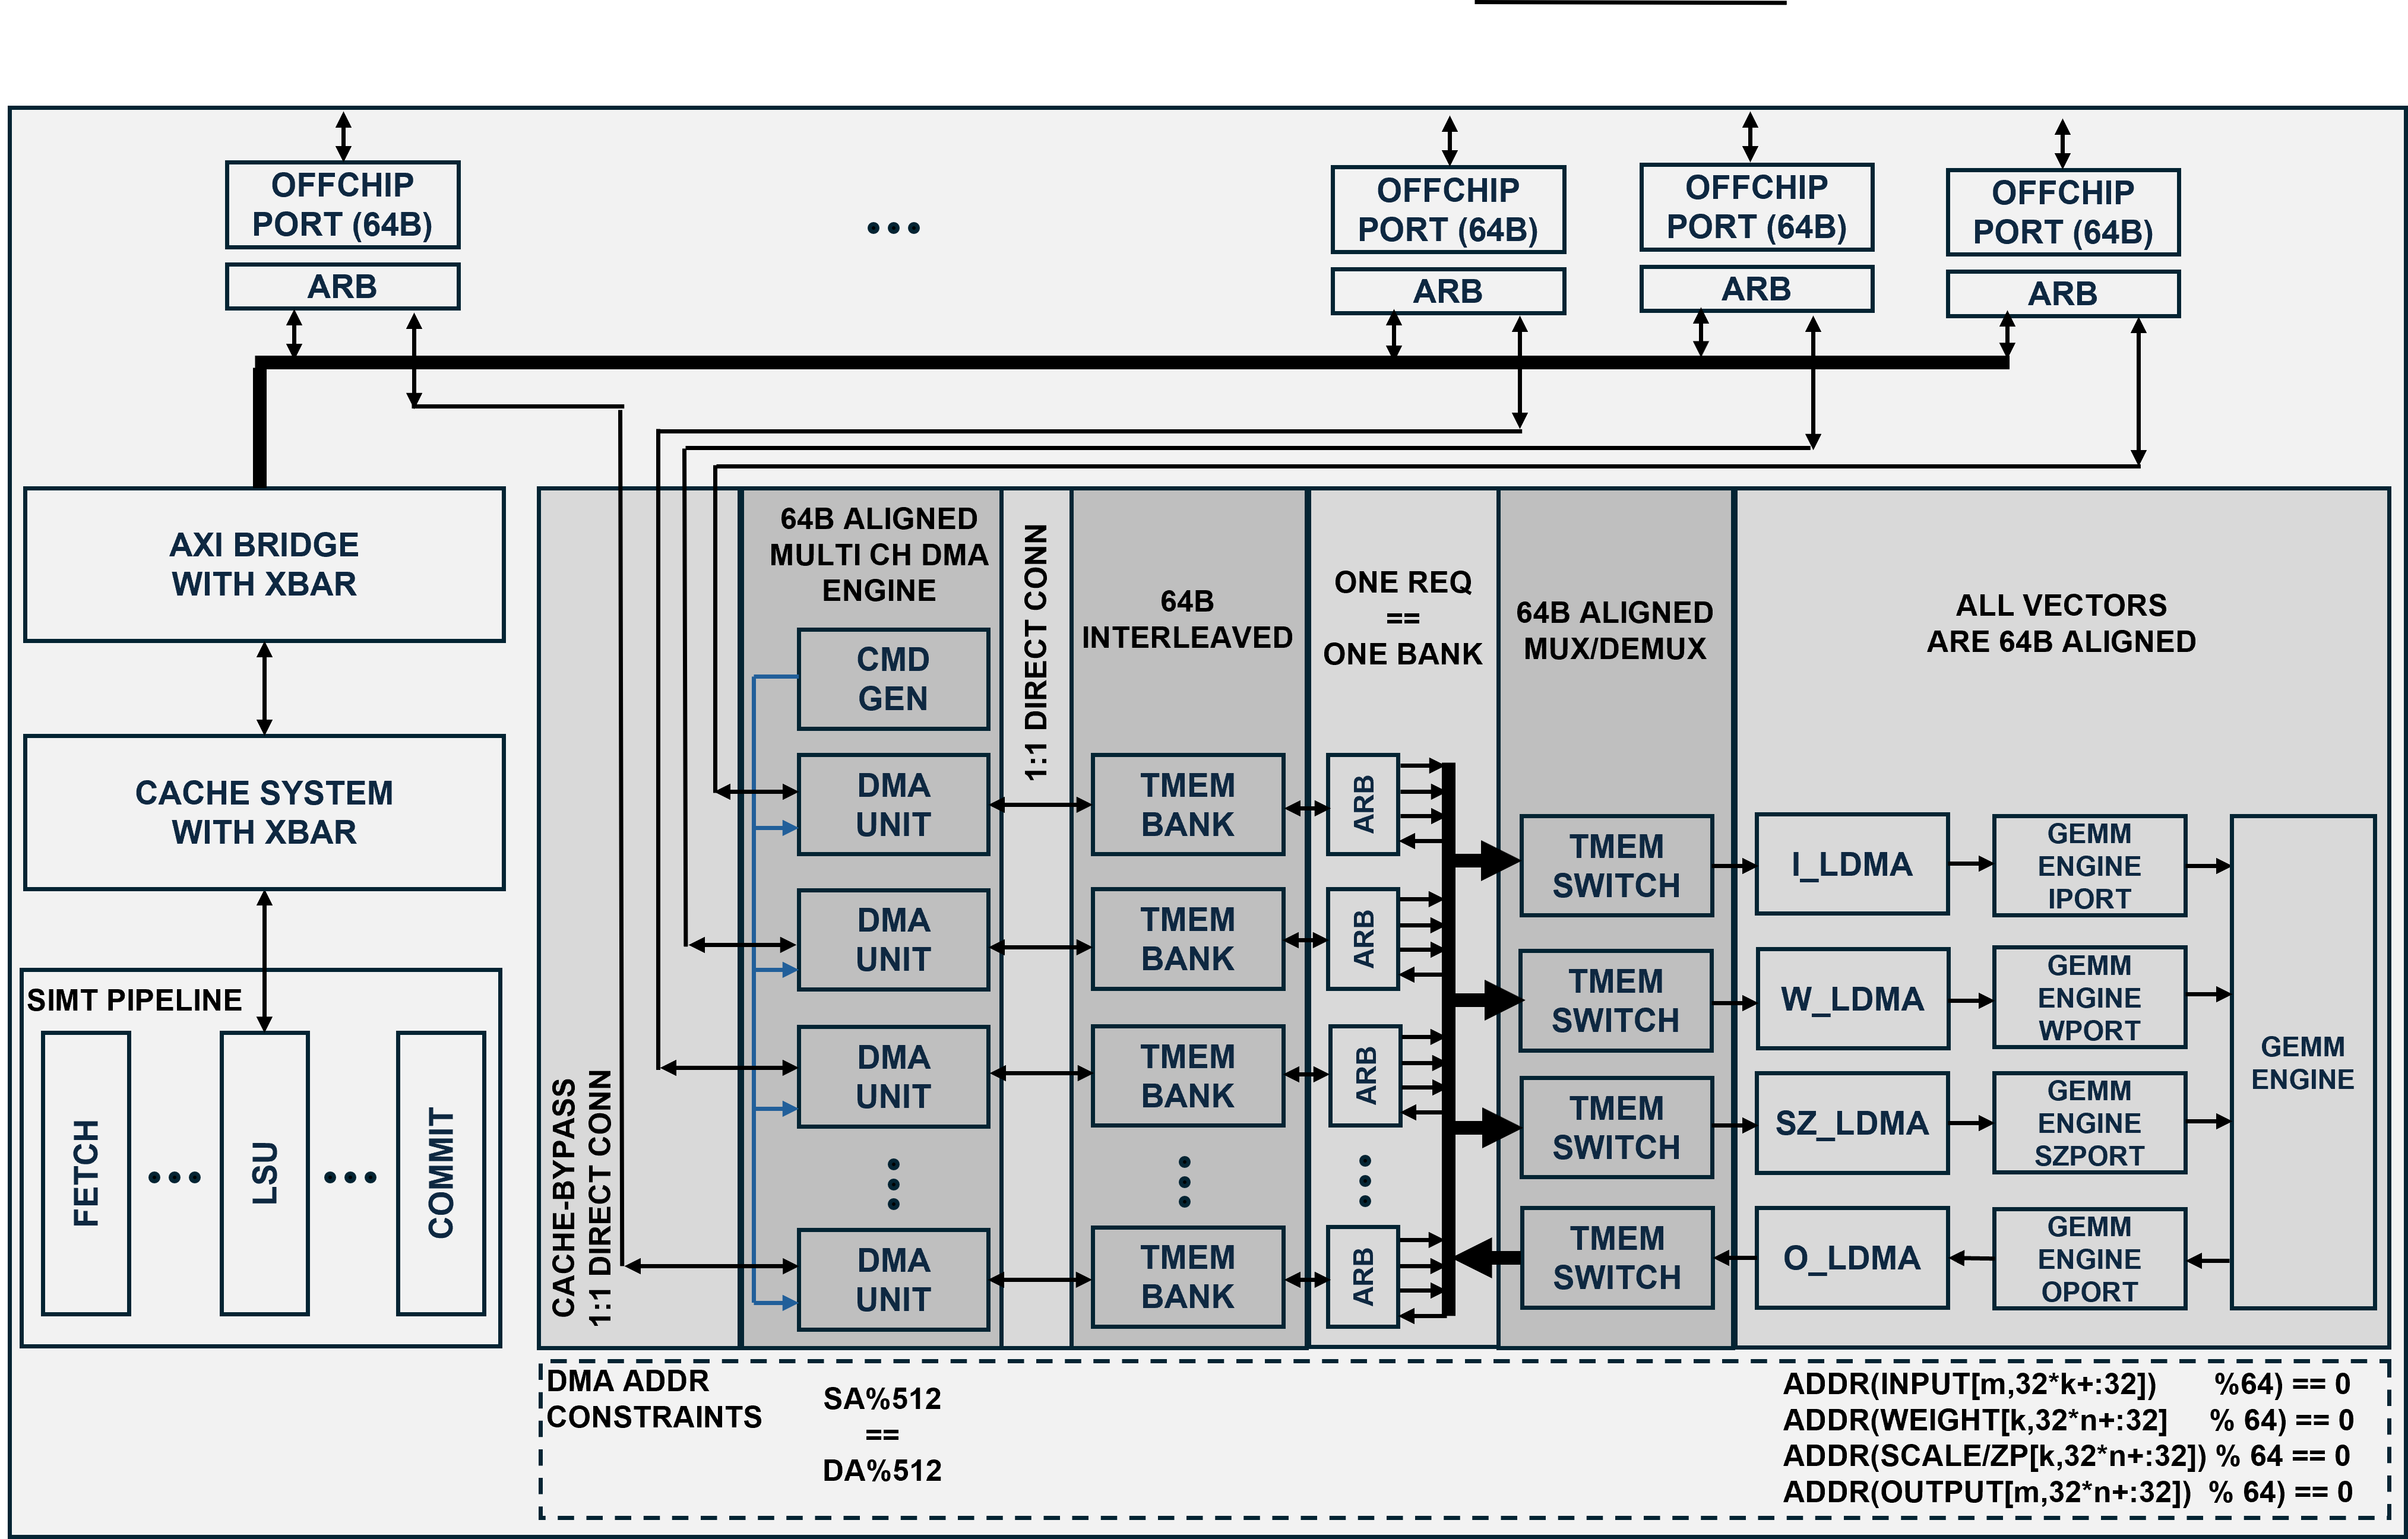
\includegraphics[width=0.92\linewidth]{figures/mem_sub_system.png}
%     \caption{Memory system for sustaining large \fpint{} arrays with direct tensor data movement.}
%     \label{fig:memory-system}
% \end{figure}
\begin{figure*}[t]
    \centering
    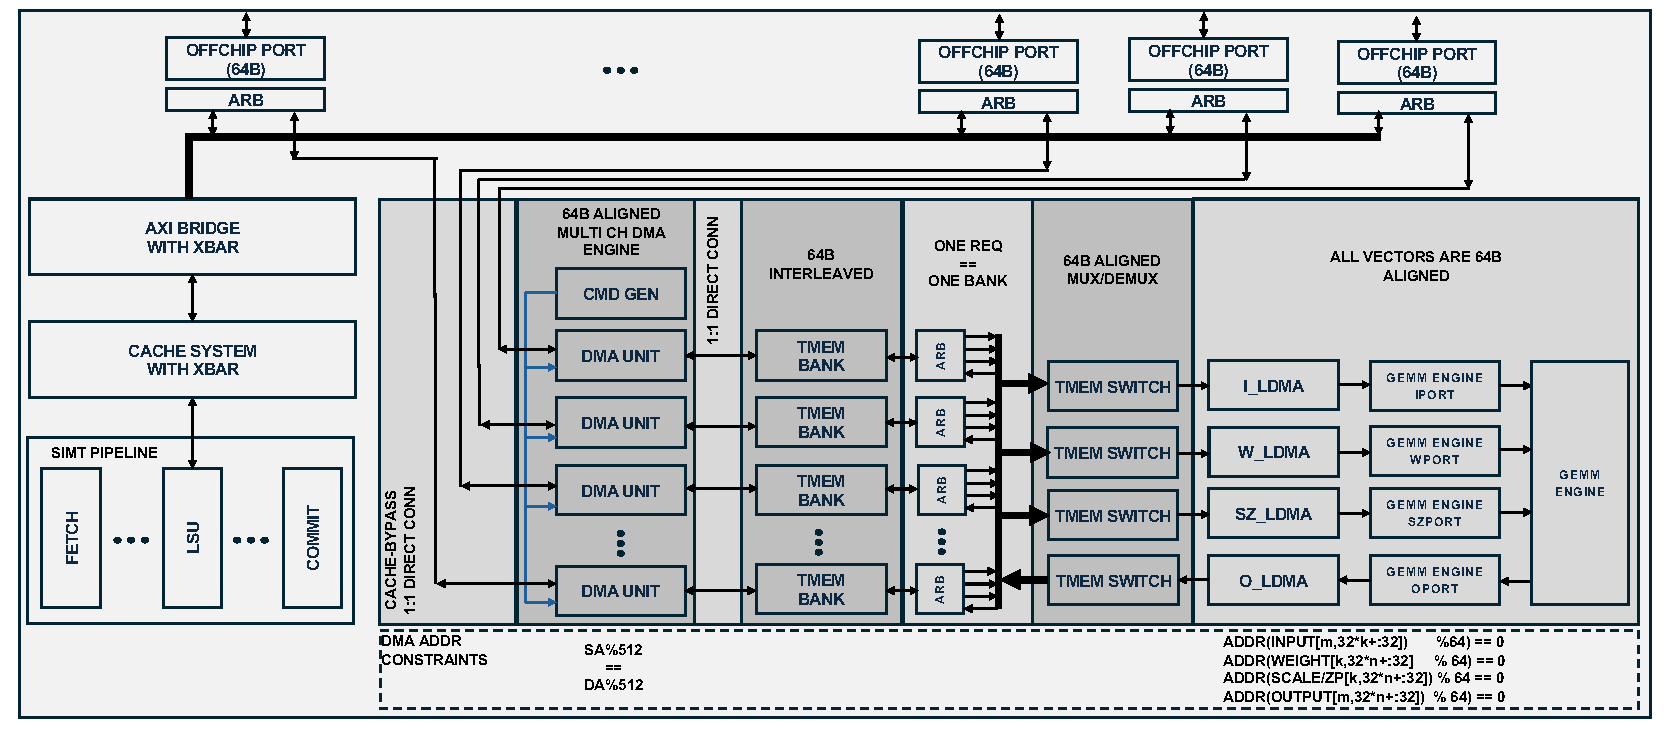
\includegraphics[width=0.96\textwidth]{figures/mem_sub_system.pdf}
    \caption{Memory system for sustaining large \fpint{} arrays with direct tensor data movement.}
    \label{fig:memory-system}
\end{figure*}
Tensor traffic also bypasses the cache hierarchy. Routing it through the cache would force it onto general-purpose paths shared with cache banks, local memory, and SIMT load/store, and scaling those paths to the operand bandwidth of an \fpint{} MXU would once again make crossbar and multi-bank arbitration costs the bottleneck. \ours{} therefore lets the tensor DMA move data directly from HBM pseudo-channels to tensor memory banks. This choice reduces cache pollution and port conflicts with SIMT memory traffic, and allows the tensor path to be scaled with a simple interconnect. In return, since the cache-bypassed path operates outside the coherent cache protocol, the hardware does not automatically guarantee coherence between SIMT cache state and tensor memory movement. As described in Section~\ref{sec:runtime-section}, \ours{} resolves this issue through explicit synchronization in the GEMM kernel.
Overall, the proposed memory system prevents the array-level efficiency of the \fpint{} unit from being lost to an operand-supply bottleneck. By combining descriptor-driven GEMM execution, partitioned tensor storage, a direct-connected DMA path, and cache bypass, it separates traffic that needs general-purpose flexibility from high-bandwidth tensor traffic.

\section{Layout transformation and runtime optimization}
\label{sec:runtime-section}

\begin{figure}[t]
    \centering
    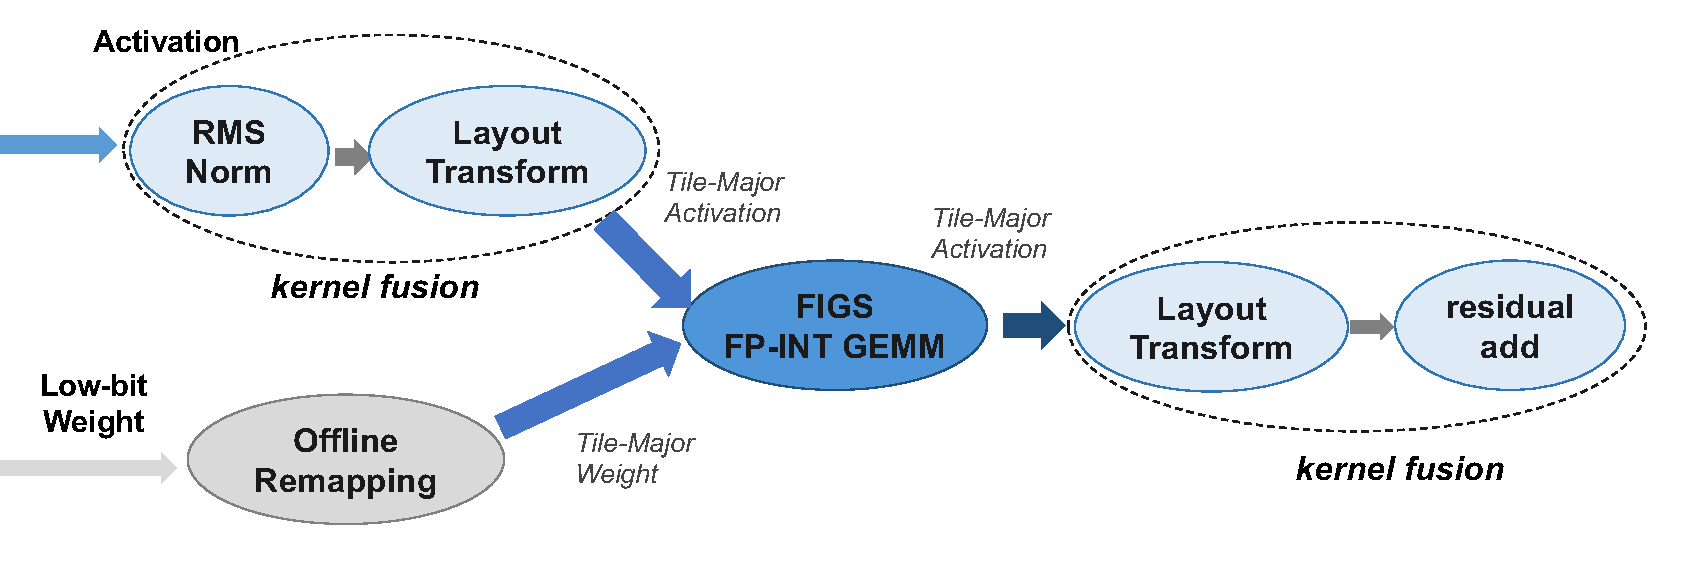
\includegraphics[width=0.92\linewidth]{figures/layout_fusion.pdf}
    \caption{Fused layout transformation for feeding cache-bypassed tensor DMA. The figure is simplified and shows representative fusion sites only.}
    \label{fig:fuse_layout_transform}
\end{figure}

The memory system of the previous section simplifies the hardware fabric at the cost of three software-visible constraints: address alignment, bank mapping, and non-coherent DMA. The software layer of \ours{} satisfies these constraints with little effort by exploiting the regular tile-access pattern of GEMM, using a fused tile-major layout transform and alignment-aware memory allocation. The key idea is that, instead of relying on a complex interconnect in hardware, the software keeps both the tensor layout and the location at which the tensor is placed in memory in a form that the hardware can consume most efficiently.
 
\textbf{Tile-major Layout and Aligned Allocation:}
\ours{} meets the constraints of Section~\ref{sec:memory-system} by changing the tensor layout to a tile-major form, choosing tile sizes appropriately, and jointly controlling the base address at which the tile is allocated in memory.
 
\ours{} launches a layout-transform kernel from SIMT to convert the input and output tensors of every GEMM into a tile-major format. During a GEMM, the tiles moved from HBM to TMEM have tile sizes $M_T$, $K_T$, $N_T$, while the tiles exchanged between TMEM and the GEMM engine have tile sizes $MT_{mxu}$, $KT_{mxu}$, $NT_{mxu}$. We set each tile size to a multiple of the modulus required by the constraints in Section~\ref{sec:memory-system} and store the elements within a tile contiguously, so that the constraints are met by construction.
 
\ours{} extends the Vortex runtime so that, in addition to the existing alignment option on the requested size, memory allocation accepts an alignment constraint on the base address as well. The runtime then applies the alignment constraint jointly to HBM and tensor-memory allocations so that Eq.~\ref{eq:hbm_tmem_addr_constr} is satisfied. Kernels do not pass arbitrary pointers to the DMA engine; instead, they use aligned tensor objects and tile descriptors guaranteed by the runtime. Under this contract, the DMA only needs to handle aligned bursts and requires neither a wide barrel shifter nor a general crossbar. Once the constraint is resolved at allocation time, Eq.~\ref{eq:hbm_tmem_addr_constr} continues to hold as long as the tile-major layout and an appropriate tile size are preserved.
 
Tile-major layout and alignment not only enable a simple interconnect but also substantially improve DMA efficiency itself. DMA efficiency is largely determined by how large a contiguous segment a single request can move. When the response latency is long and small requests are issued repeatedly, bubbles appear between requests and theoretical bandwidth is hard to translate into actual throughput. Transferring a tile in row-major or column-major order therefore introduces bubbles between rows or columns, and on a deeply pipelined long-latency path this causes DMA efficiency to drop sharply. With a tile-major layout, the data the DMA must fetch reside at contiguous addresses, so the entire DMA operation can be completed with a single command. The DMA engine in \ours{} contains multiple DMA units that auto-generate addresses from stride and bound information to move data. The engine receives a descriptor, and its controller partitions the target tensor region across the DMA units to fetch the tensor in parallel. Here again, the simple interconnect and the channel-to-bank mapping of \ours{} minimize the mux, demux, and other logic required inside the controller and the DMA engine.
 
\textvf{Explicit Ownership and Synchronization:}
Cache-bypassed DMA raises a coherence concern. In a \wkv{} GEMM kernel, however, the SIMT pipeline and the \fpint{} engine never access the same in-flight tile arbitrarily at the same time; ownership of each tensor tile is well-defined per phase. SIMT code or the runtime prepares descriptors and metadata; the DMA moves a tile from HBM into tensor memory; the MXU consumes tensor memory and accumulator memory; and the SIMT pipeline reads results only after accumulation has completed. At the points where ownership transfers between the SIMT and tensor paths, the kernel inserts explicit fences or synchronization to guarantee visibility. In other words, \ours{} resolves coherence not through a complex hardware protocol, but through tile-level explicit synchronization.
 
\textbf{Fused Layout Transformation:}
Running the layout transform as a stand-alone kernel would let a separate memory pass cancel out the gains obtained on the tensor path. \ours{} therefore fuses the layout transform into surrounding kernels such as Q/K/V projection, quantization, GEMM preparation, and output movement, hiding the transform cost within them. As a result, tensors are kept in a DMA-friendly layout from the moment they are written to HBM, and the alignment required by the direct-connected path is satisfied inside steady-state kernel execution.


\section{Evaluation}

\subsection{Methodology}
\textbf{Hardware Evaluation Setup}
We compare four hardware candidates.

\begin{itemize}
    \item \textit{C1: FP TCU based GPU.}
    Implemented by enabling an FP$\times$FP TCU on Vortex.
    C1 executes all GEMM operations on the FP TCU after
    dequantizing the INT-quantized operands on the SIMT core.

    \item \textit{C2: Linear Only FP$\times$INT GPU.}
    We add a decoupled \fpint{} MXU on top of C1.
    The QKV generation and the FFN linear projections are
    executed on the \fpint{} MXU, while the $QK^T$ and PV
    operations of attention are executed on the FP TCU.
    C2 represents prior work such as FIGNA/FIGLUT/LUT-TC
    that accelerates only linear operations with \fpint{}.

    \item \textit{C3: Naive WKV GPU.}
    Both linear layers and attention $QK^T$/PV operations are
    executed on the \fpint{} MXU. The memory subsystem
    remains naive.

    \item \textit{C4: FIGS.}
    Final design with \fpint{} execution for both linear and
    attention kernels, together with the memory subsystem,
    runtime, and layout optimizations.
\end{itemize}

\begin{figure}[t]
    \centering
    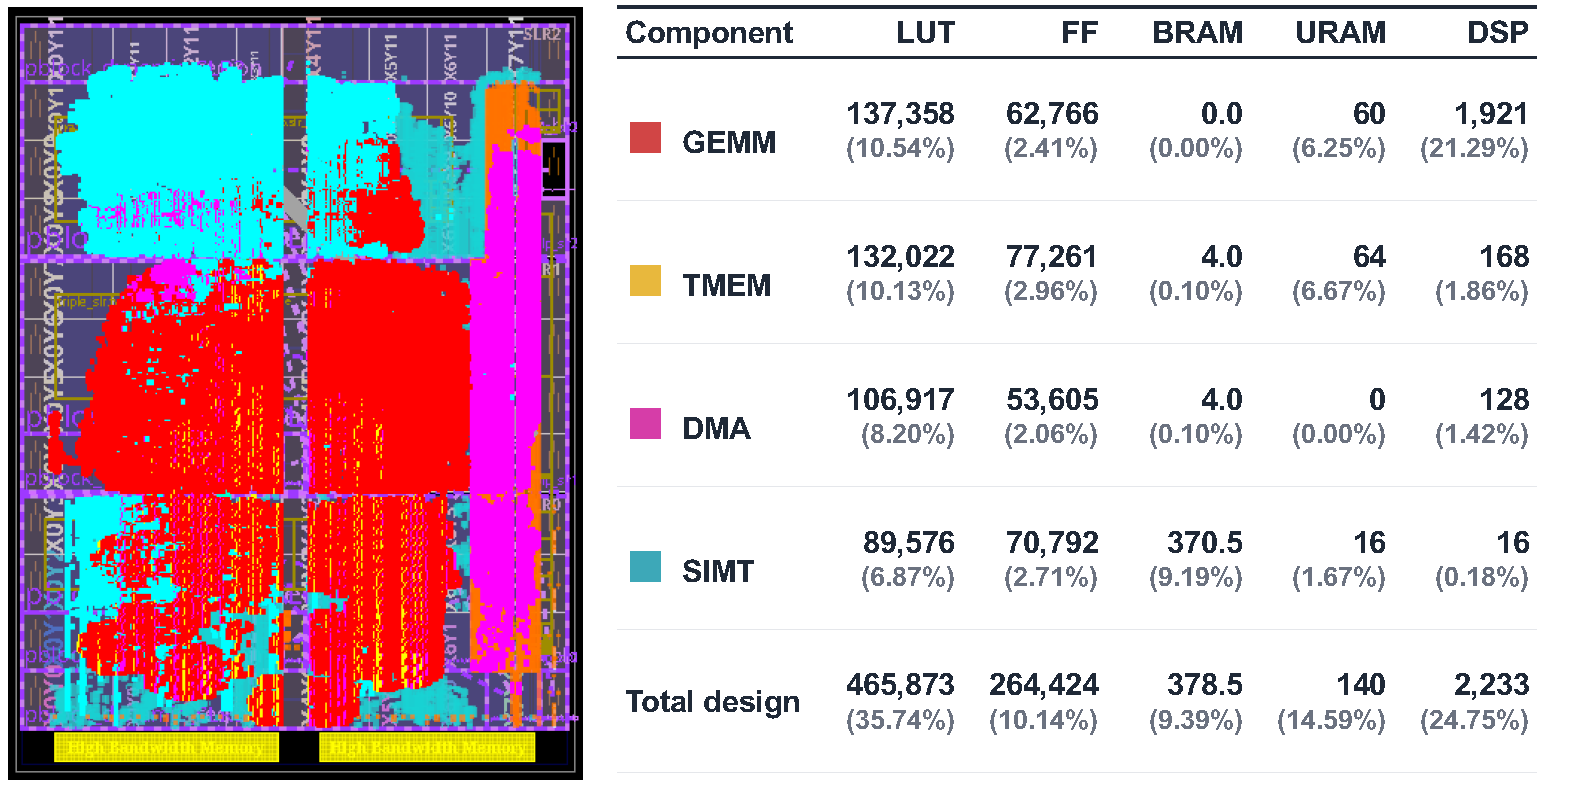
\includegraphics[width=\linewidth]{figures/fpga_floorplan.pdf}
    \caption{Floorplan and resource breakdown of \Cfou{} on the Alveo U55C.}
    \label{fig:floorplan}
\end{figure}

Table~\ref{tab:candidates} lists the parameters of each candidate. All candidates use a single core, with 4 warps per core and 32 threads per warp. The TCU size is set to 8x4x4 according to the thread count. The \fpint{} GEMM engine uses a 32x32 array. The cache size is configured identically across all candidates, and the local memory size is also configured identically. When tensor memory is present, the combined size of local memory and tensor memory is set equal to the local memory of the other candidates. All performance evaluations are conducted on real hardware: every candidate is placed-and-routed and deployed on a Xilinx Alveo U55C FPGA, and all reported numbers are measured from on-board execution rather than from RTL simulation. Resource usage table and floorplan of our final design(C4) is displayed in figure \ref{fig:floorplan}


Each candidate takes the same \wkv{} quantized model as input, differing only in which operations are mapped to which hardware path. Area is measured after synthesis at a 100MHz target on a 28nm node using Synopsys Design Compiler. Power is measured by placing-and-routing the candidates on an FPGA at a 100MHz target and then measuring board power with xrt-smi while running the kernels multiple times; dynamic power is obtained by subtracting the idle power from the measured power.

When reporting performance, we normalize by area or power for a fair comparison.

\begin{table}[t]
\centering
\caption{Hardware candidates for evaluation.}
\label{tab:candidates}

\footnotesize
\setlength{\tabcolsep}{2pt}

\begin{tabular}{
p{0.14\columnwidth}
p{0.14\columnwidth}
p{0.09\columnwidth}
p{0.10\columnwidth}
p{0.12\columnwidth}
p{0.12\columnwidth}
}
\toprule
Candidate & Name & Num Warps & Num Threads & FP TCU Size & \fpint{} MXU Size \\
\midrule
C1 & \Cone{} & 4 & 32 & 8x4x4 & -- \\
C2 & \Ctwo{} & 4 & 32 & 8x4x4 & 32x32 \\
C3 & \Cthr{} & 4 & 32 & -- & 32x32 \\
C4 & \Cfou{} & 4 & 32 & -- & 32x32 \\
\bottomrule
\end{tabular}
\end{table}

\textbf{Workloads}
The evaluation covers prefill, generation, and end-to-end inference. We primarily evaluate Llama2-7B, quantized with SpinQuant to 4-bit weights and KV. The quantization options follow the default parameters of SpinQuant.

\textbf{Software Implementation}
The kernel launch code is implemented in C++ using the Vortex runtime, and the kernels are implemented natively in C++ for Vortex. Vector operations are implemented in an SPMD style, as in conventional GPU kernels. For GEMM operations, kernels that use the FP TCU rely on the TCU kernels provided by Vortex, while kernels that use the \fpint{} MXU are implemented through MMIO. The kernel first writes the matrix size, the transpose flag of the RHS, and the quantization direction to predetermined addresses, then invokes the GEMM node; it subsequently polls a status register exposed through MMIO until the GEMM operation completes. The implemented kernel launch code and kernels are integrated with the deep learning frontend through PyTorch's PrivateUse1 backend; tensors are copied to the accelerator DRAM via the \texttt{.to} method, similar to the CUDA flow, after which PyTorch operators are called and dispatched to the Vortex kernels. This stack allows \ours{} to be evaluated not as a bare GEMM microbenchmark but within a real LLM inference graph, where the memory system, runtime layout, and native \fpint{} attention support all operate together.

\subsection{End-to-End Performance Improvement}

\begin{figure*}[t]
    \centering
    \includegraphics[width=\textwidth]{figures/main_all/bar_total_p50_us.png}
    \caption{element kernel included}
    \label{fig:main_result}
\end{figure*}

Figure~\ref{fig:main_result} shows the area/power-normalized performance for C1--C4 when running end-to-end inference of Llama2-7B. For prefill we use a batch size of 1 and sweep the sequence length from 512 to 16k; for decode we sweep the batch size over 1, 8, and 64 while sweeping the sequence length from 512 to 16k. In prefill, for both area- and power-normalized performance, \ours{} is on average x$\times$ and x$\times$ higher than the baseline across all test cases. The improvement of \ours{} decreases as the sequence length grows, because the softmax latency increases as $O(N^2)$ and the GEMM portion shrinks accordingly.

Comparing C1 and C2, C1 is better in some cases while C2 is better in others. C2 approaches C1 in efficiency as the sequence length grows: as the sequence length increases, attention dominates, but C2 handles attention with the FP TCU while using \fpint{} for the linear projections. Because it must carry both the FP TCU and the \fpint{} MXU, C2 becomes less efficient than the baseline C1 within the same area or power budget. This suggests that designs that support only linear operations with \fpint{}, such as LUT-TC and FIGNA, can in fact become less efficient in the long-sequence regime. C3 executes both linear and attention with \fpint{}, eliminating the FP TCU overhead, and is therefore better than C2 in essentially all cases (with one exception, decode at BS=64). However, because its memory subsystem and DMA are integrated naively without optimization, C3 cannot sustain high \fpint{} utilization and is consistently lower than C4 in all cases.

In decode, \Cfou{} is also the best in all cases, with area- and power-normalized performance higher by x$\times$ and x$\times$ on average, respectively. The improvement of C4 grows as the sequence length increases. The reason is xxx.

Table~\ref{tab:layout-transform-overhead} shows the overhead of the layout transform kernel used to make the GEMM input and output tensors GEMM-friendly. Performing the layout transform as a standalone kernel incurs an overhead of x\%, while fusing it with the kernels immediately before and after the GEMM reduces the overhead to about 1\%, rendering it nearly negligible.

\begin{table}[H]
\centering
\caption{Overhead of fused layout transform is very low.}
\label{tab:layout-transform-overhead}
\begin{tabular}{p{0.14\linewidth}p{0.24\linewidth}p{0.24\linewidth}p{0.14\linewidth}p{0.14\linewidth}}
\toprule
%kernel & plain kernel & after fusion & overhead(\%) \\
kernel & sequence length & hidden dim & overhead(\%) \\
\midrule
%rmsnorm &  {3745.2us} & {3750.46us} & {+0.1\%}\\
%silu &  {16337.69us} & {16556.56us} & {+1.3\%}\\
rmsnorm &  8 \todo{다른 length도 실험} & 4096 & {+0.1\%}\\
silu &  8 & 11008 & {+1.3\%}\\
\bottomrule
\end{tabular}
\end{table}

\subsection{Performance Breakdown}

Figure~\ref{fig:breakdown} shows the area/power-normalized performance breakdown of the GEMM operations contained in the linear projections and attention. Specifically, for prefill and decode at a short sequence (s512) and a long sequence (s16384), it decomposes the ISO-AREA and ISO-POWER normalized latency of the linear projections (qkv\_proj, out\_proj, ffn) and attention (qk, pv) GEMMs across C1--C4. The purpose of this breakdown is to isolate which operation path produces the end-to-end speedup of Figure~\ref{fig:main_result}, and which candidate removes which bottleneck.
Across all sequence lengths, the linear projections drop sharply from C1 to C2, because the FP$\times$INT MXU provides more MACs in the same area. This gain is most pronounced in the compute-intensive prefill regime. Under area normalization, however, C2 carries both FP MACs and FP$\times$INT MACs, and thus performs worse than the baseline at large sequence lengths: as the sequence length grows, the attention (qk + pv) operations that C2 cannot reduce dominate, which is also visible in the graph. Under power normalization, by contrast, even though C2 carries both FP and FP$\times$INT MACs, only one path is exercised at any given time, so C2 looks better than the baseline. C3 and C4 route attention through the FP$\times$INT path as well, and therefore show strong improvements over the baseline across all GEMM paths; in particular, they exhibit a large gap over C2 in the long-sequence regime.

\begin{figure*}[t]
    \centering
    \includegraphics[width=\textwidth]{figures/main_all_gemm_only/bar_total_p50_us.png}
    \caption{element kernel not included}
    \label{fig:breakdown}
\end{figure*}

\begin{figure*}[t]
    \centering
    \includegraphics[width=\textwidth]{figures/energy_per_token/energy_per_token.png}
    \caption{energy per tokens}
    \label{fig:energy_per_token}
\end{figure*}

\subsection{Accuracy}

\begin{table*}[t]
\centering
\caption{Zero-shot accuracy and ppl comparison of W4A16KV4 variants.}
\label{tab:accuracy}

\resizebox{\textwidth}{!}{
\begin{tabular}{lcccccccccc}
\toprule
& ARC-c & ARC-e & BoolQ & HellaSwag & OpenBookQA & PIQA & SocialIQA & WinoGrande & Zero Shot Avg. & wiki2 \\
\midrule
W4A16KV4 & 44.20 & 73.15 & 76.85 & 75.35 & 42.60 & 78.56 & 45.24 & 68.82 & 63.10 & 5.59 \\
W4A16KV4 (linear) & 44.37 & 72.98 & 76.24 & 75.34 & 43.20 & 78.40 & 45.29 & 69.22 & 63.13 & 5.59 \\
W4A16KV4 (attn) & 44.03 & 73.32 & 76.82 & 75.23 & 43.20 & 78.56 & 44.73 & 68.19 & 63.01 & 5.59 \\
\rowcolor{gray!12}
W4A16KV4 (linear + attn)
& 44.03 & 73.02 & 77.13 & 75.22 & 44.20 & 78.78 & 45.24 & 69.53 & 63.39 & 5.59\\
\bottomrule
\end{tabular}
}
\end{table*}


This experiment examines the impact of WKV quantization on model accuracy. Because the goal of our hardware is to efficiently execute the operations of a quantized model, it must preserve the same numerical behavior as the baseline when the same quantization algorithm is used, and the hardware must not introduce any new accuracy degradation. Table~\ref{tab:accuracy} compares the zero-shot accuracy of four variants that differ in the scope of operations to which the FP$\times$INT path is applied, on Llama2-7B quantized with SpinQuant to W4A16KV4. It reports the case where the path is applied only to the linear layers (linear), only to the $QK^T$ and $PV$ of attention (attn), and to both (linear + attn), alongside the full WKV quantization (W4A16KV4). The average accuracy over the eight downstream tasks is 63.10, 63.13, 63.01, and 63.39, respectively, so all variants stay within 0.4\%p of one another. The target configuration of this work (linear + attn), which executes attention in FP$\times$INT as well, in fact achieves the highest average at 63.39, and on individual tasks such as ARC-c, ARC-e, BoolQ, and HellaSwag it remains consistently comparable to or better than the other variants. This result shows that the FP$\times$INT MXU does not incur accuracy loss even when it natively processes quantized operands on both the linear and attention paths. In other words, the system-level performance improvement proposed in this work is obtained without sacrificing numerical accuracy, confirming that the accuracy determined by the quantization scheme and the hardware acceleration are independent of each other.

\subsection{Breakdown and Overhead Analysis}

\paragraph{Array-level efficiency}
We measure how much higher compute density and energy efficiency the \fpint{} array provides compared to the FP$\times$FP TCU. It is x$\times$ better than FP$\times$FP. The overhead relative to the WoQ unit is x, which is very small. Considering that attention can be executed in FP$\times$INT, the WKV GEMM unit is effectively x$\times$ more efficient than the WoQ GEMM unit (Figure~\ref{fig:arr-level-break}).

\begin{table}[H]
\centering
\caption{Relative array-level comparison. 28n tech. 100M. 32x32 size array}
\label{tab:array-level}
\begin{tabular}{p{0.22\linewidth}p{0.20\linewidth}p{0.20\linewidth}p{0.20\linewidth}}
\toprule
Unit & Precision & TOPS/mm$^2$ & TOPS/W \\
\midrule
FP TCU & FP$\times$FP & 1.0 & 1.0 \\
WoQ \fpint{} MXU & FP$\times$INT & 2.32 & 3.04 \\
WKV \fpint{} MXU & FP$\times$INT & 2.21 & 2.97 \\
\bottomrule
\end{tabular}
\end{table}

\begin{figure}[t]
    \centering
    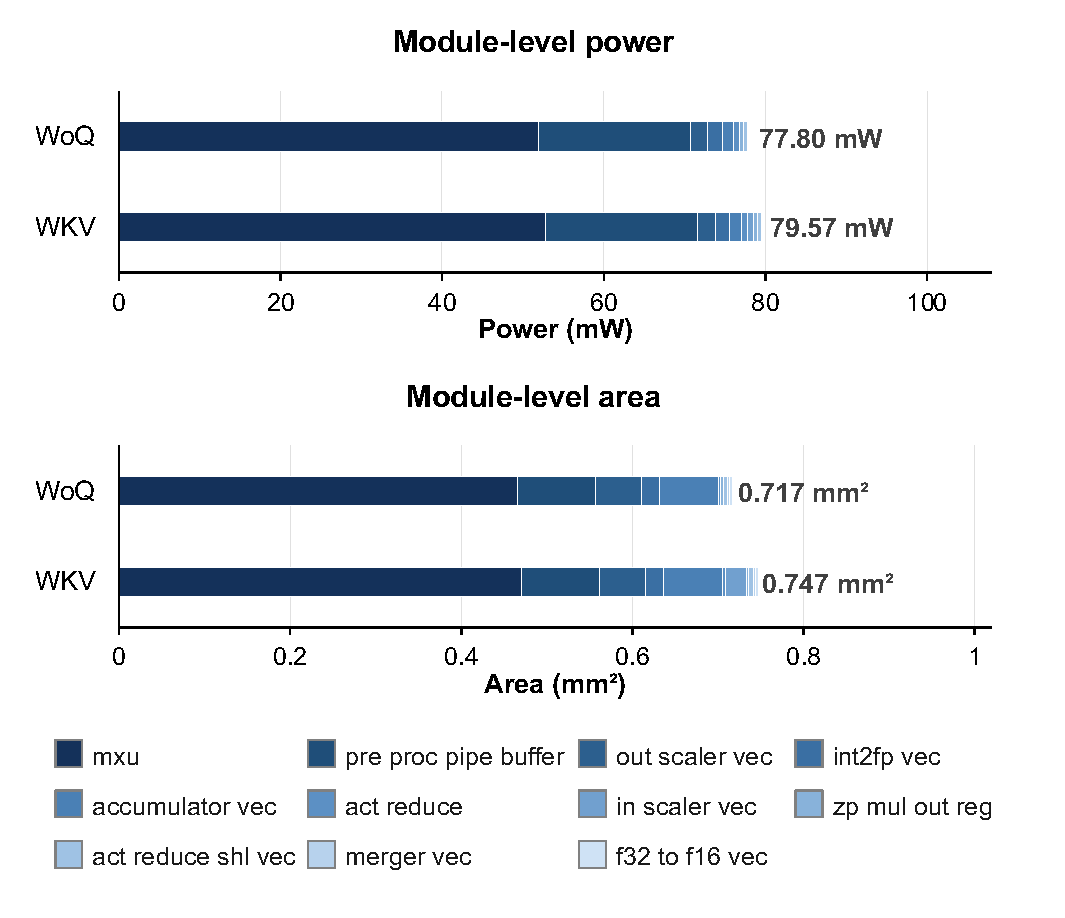
\includegraphics[width=\linewidth]{figures/wkv_vs_woq_overhead_cropped.pdf}
    \caption{WoQ에 비해 WKV의 gemm unit level에서의 overhead가 작다는 것을 보여주자.}
    \label{fig:arr-level-break}
\end{figure}

\paragraph{Area breakdown}
This is the area breakdown of \ours{} (Figure~\ref{fig:area-breakdown}). The overhead related to interconnection scaling is small.

\begin{figure}[htbp]
    \centering
    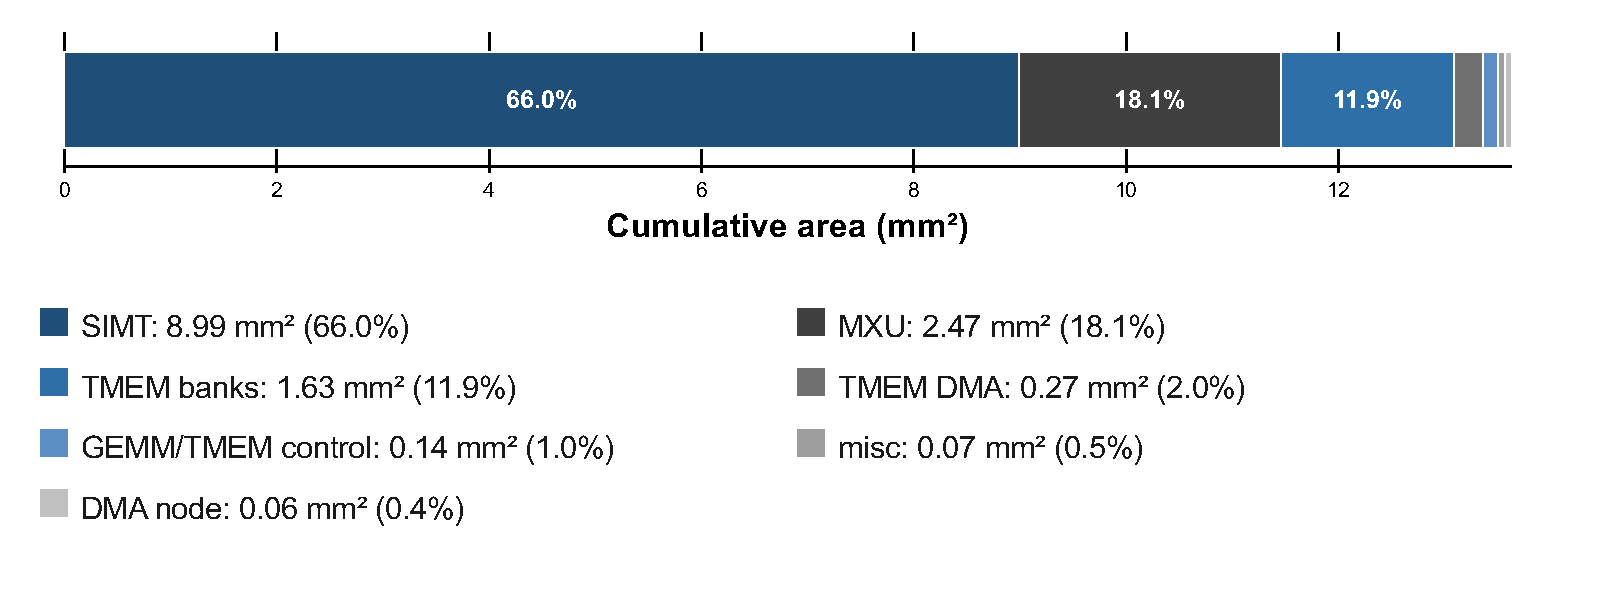
\includegraphics[width=\linewidth]{figures/area_breakdown.pdf}
    \caption{simple interconnect 덕분에 dma와 interconnect 쪽에서 overhead가 거의 없다.}
    \label{fig:area-breakdown}
\end{figure}

\section{Conclusion}
This paper argues that the benefit of WKV quantization cannot be fully realized by reducing memory traffic alone. In WKV-quantized LLM inference, the recurring compute pattern is \fpint{} GEMM across both the linear layers and the KV-attention path. Existing GPU kernels give up the compute-side efficiency because they lack a \fpint{} datapath, while prior \fpint{} hardware primarily accelerates linear layers and leaves long-sequence attention and system-level data feeding as bottlenecks.

We presented \ours{}, a Vortex-based hardware/software system that turns \fpint{} array efficiency into end-to-end LLM inference performance. \ours{} introduces an RHS-axis-reconfigurable \fpint{} MXU that supports both quantization directions and RHS load orientations, enabling native \fpint{} attention by executing both QK$^T$ and PV on the \fpint{} datapath instead of falling back to the FP path. To sustain high utilization on the larger array, \ours{} decouples GEMM execution from the SIMT pipeline, separates tensor and accumulator storage from general-purpose local memory, and uses direct-connected, cache-bypassed tensor data movement to avoid crossbar scaling costs. The resulting address and bank-mapping constraints are handled in software through tile-major layout, aligned allocation, explicit synchronization, and fused layout transformation.

Our evaluation on an end-to-end Vortex stack shows that these components are complementary. A linear-only \fpint{} design improves the linear layers but remains limited by attention at long sequence lengths; adding native \fpint{} attention removes that bottleneck, and the optimized memory subsystem and runtime support are needed to preserve the utilization of the larger array. The accuracy study further shows that executing both linear and attention paths through the native \fpint{} datapath preserves the numerical behavior of the underlying WKV quantization scheme. Overall, \ours{} demonstrates that realizing the promise of \fpint{} hardware for LLM inference requires co-design across the GEMM datapath, memory system, and runtime stack, rather than an efficient array alone. With this co-design, \ours{} improves end-to-end LLM inference performance by x$\times$ and energy efficiency by x$\times$ over the conventional GPU baseline.



\section*{Acknowledgements}
This document is an updated version of HPCA 2022 and 2023, which, in
turn, has been derived from two previous conferences, in particular
HPCA 2021 and MICRO 2021, which, in turn, are derived from past MICRO,
HPCA, ISCA, and ASPLOS conferences.

%%%%%%% -- PAPER CONTENT ENDS -- %%%%%%%%


%%%%%%%%% -- BIB STYLE AND FILE -- %%%%%%%%
\bibliographystyle{IEEEtranS}
\bibliography{refs}
%%%%%%%%%%%%%%%%%%%%%%%%%%%%%%%%%%%%

\end{document}

